\chapter{Porównanie metod detekcji - eksperymenty}

Podczas eksperymentowania z~różnymi algorytmami i~metodami detekcji,
rozpoznawania obiektów oraz obróbki obrazów powstało
oraz zostało wstępnie przetestowanych wiele implementacji
najbardziej obiecujących rozwiązań. Wiele z~nich już w~trakcie
pierwszych testów prezentowały skuteczność na niezadowalającym
poziomie. Inne były zupełnie niezwiązane z~zagadnieniem,
a~jeszcze inne zostały popełnione aby zachować pozory użyteczności 
i~przydatności rozwiązania omawianego problemu w~codziennym życiu.

W~tym rozdziale przedstawione i~pokrótce opisane zostały kroki podjęte
w~celu znalezienia najbardziej optymalnego rozwiązania postawionego 
problemu. 
W~pierwszej kolejności przedstawiono kilka prób, które ze względu
na niezadowalające wyniki lub trudności w~implementacji
nie zostały uwzględnione w~rozwiązaniu końcowym. W~kolejnym podrozdziale
pokazano szereg prób weryfikacji skuteczności i~optymalizacji 
poszczególnych kroków ostatecznego algorytmu. W~podsumowaniu uwzględniono
częściowo przypadkowo zidentyfikowane właściwości zastosowanych
narzędzi oraz implementacji, a także wpływ tychże odkryć na ostateczny
kształt finalnego rozwiązania.

\section{Algorytmy i~narzędzia nie wykorzystane w~rozwiązaniu końcowym}

W~tym podrozdziale przedstawione zostały próby, których wykonanie
skutkowało jedynie zwiększeniem świadomości na temat zagadnienia.
Główną przyczyną niewykorzystania zamieszczonych tutaj pomysłów
była niepewność co do skuteczności, bądź wydajności rozwiązania końcowego
które miało by być na nich oparte.

Pozostałe przyczyny to m.in. niedostosowanie rozważanego rozwiązania
do omawianego problemu. Ostatecznie zbyt duży nakład pracy, która
byłaby wymagana do dostosowania potencjalnej implementacji do
stawianych wymagań, np.: optymalizacja wysokiej złożoności obliczeniowej
lub przepisanie złożonego algorytmu na język JAVA
(w~celu uruchomienia na urządzeniu z~systemem Android)
jeżeli istniały tylko implementacje w~innych językach.

\subsection{Biblioteka OpenTLD}

Pierwszym przeciwwskazaniem do wykorzystania biblioteki OpenTLD 
był brak implementacji w~języku JAVA. Algorytm wydawał się na tyle
skomplikowany, że samo jego przeportowanie ze środowiska MatLab,
czy nawet implementacji w~C++ mogło by stanowić zakres pracy
mniejszego kalibru (inżynierskiej) lub projektu zespołowego.
Pomimo to podjęto próbę kontrolną mającą na celu sprawdzenie
skuteczności i~przydatności wspomnianego rozwiązania we wstępnej 
segmentacji - detekcji frontu autobusu - 
pierwszy krok proponowanej kaskady.

\begin{figure}[h!]
    \centering
    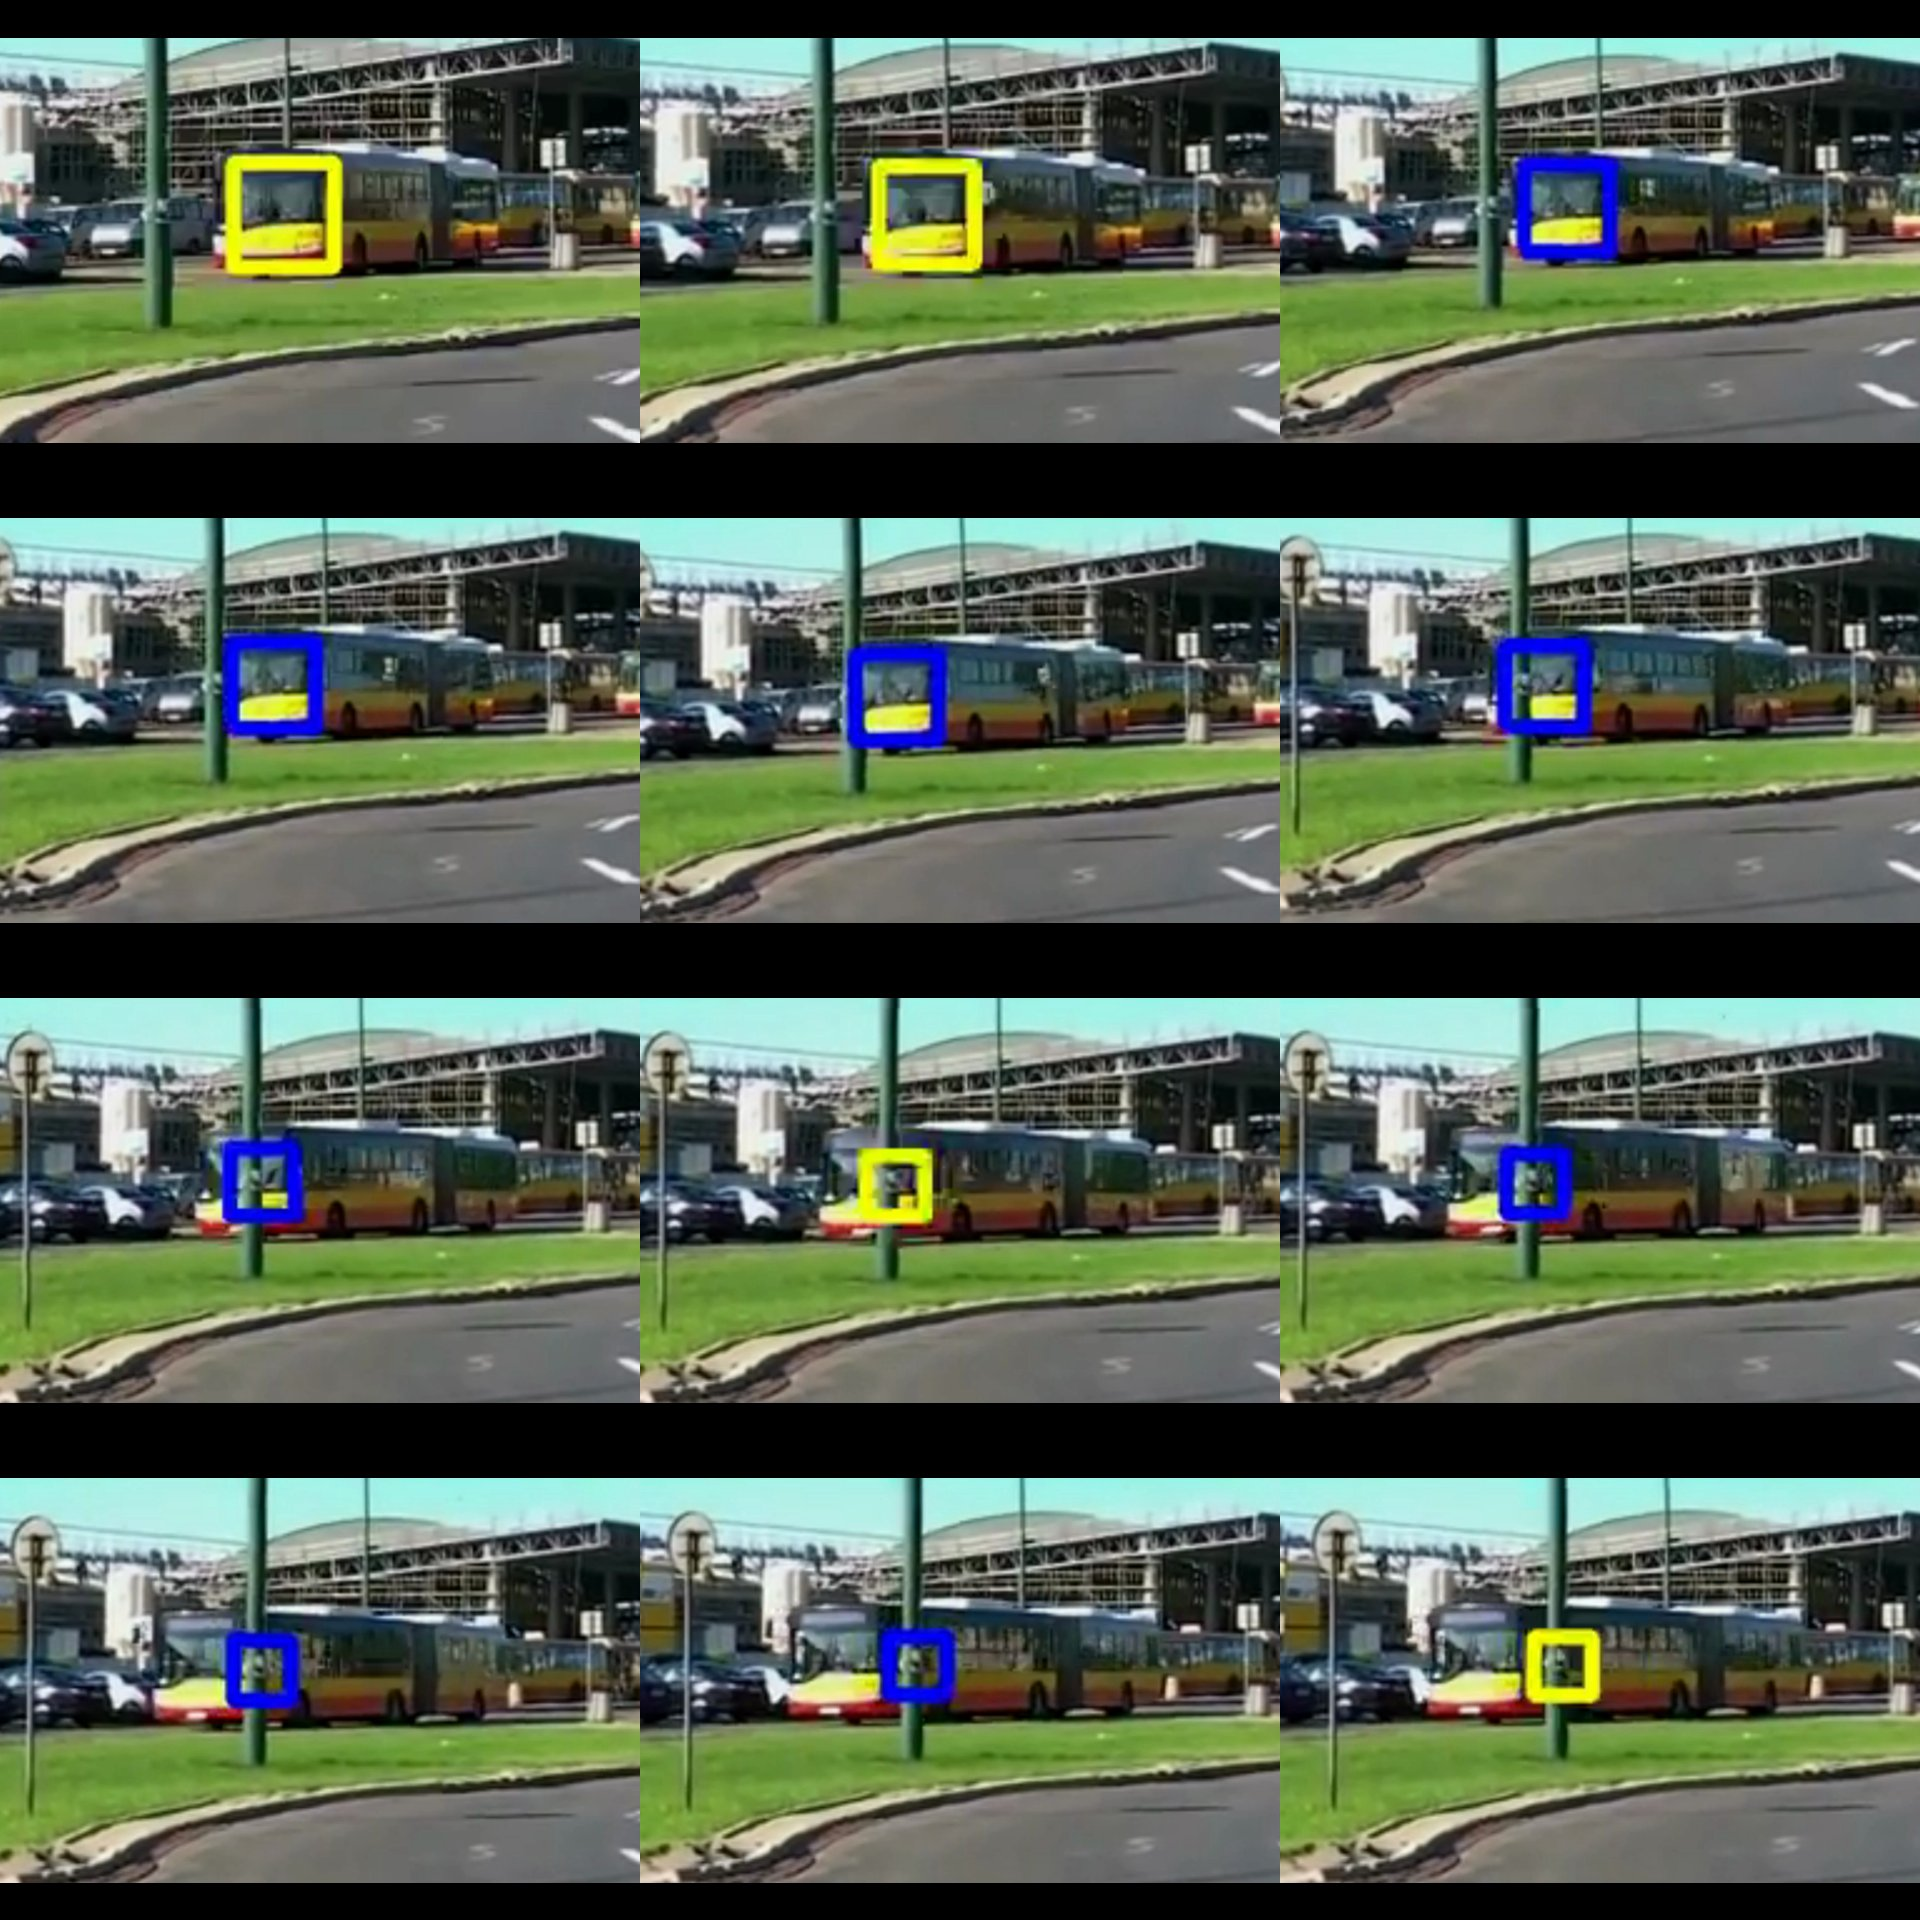
\includegraphics[width=0.9\textwidth]{img/exp_open_tld_fail}
    \caption{Niestabilność i niedokładność rezultatów uzyskanych przy
    użyciu biblioteki OpenTLD}
    \label{fig:opentld_bus_front_fail}
\end{figure}

Skuteczność wykrywania frontów autobusów (potwierdzona 
niestety jedynie w~sposób naoczny) była więcej niż zadowalająca.
Liczba trafień uzyskanych z~pojedynczego wstępnego zaznaczenia frontu
była niemal stu procentowa. Niestety dokładność wykrytych obiektów
była poniżej oczekiwanej. Standardowo zdarzały się problemy
obciętych numerów - zbyt mały czworokąt okalający. Dodatkowo
brak możliwości ingerencji w~proces uczenia detektora oraz jego
duże tendencje do ,,pływania'' skutkowały nieraz wynikami pozytywnymi
typu: lewy dolny róg frontu do 1/2 wysokości i~szerokości. 

Na rysunku \ref{fig:opentld_bus_front_fail} można zaobserwować 
zupełne zgubienie obiektu 
śledzonego - 
front autobusu - na rzecz słupa. Wynik tego eksperymentu oraz
zaobserwowany spadek wydajności - ilość obsłużonych klatek na sekundę - 
dla rosnącej liczby zebranych pozytywnych i~negatywnych próbek
(na powyższym rysunku żółte kwadraty oznaczają próbkę, która została
wykorzystana do procesu uczenia detektora) 
wpłynęły na decyzję zaprzestania dalszych testów biblioteki OpenTLD.
Ostatecznie dla jednej sesji,
nagrania długości około 5 minut, wydajność potrafiła spaść z~poziomu
początkowych 20 klatek na sekundę do nawet 2 klatek na sekundę.
Poprawa tego stanu 
rzeczy byłaby co najmniej nie na miejscu. Szczególnie, że Pan 
Zdenek Kalal wydał drugą wersję biblioteki TLD (tym razem już nie 
open), której jednym z~głównych usprawnień był właśnie znaczny 
wzrost wydajności
\cite{WEB:kalaltld2}.

\subsection{Wykrywanie linii krawężnika zatoki autobusowej}

Rozpoczynając ten podrozdział, trudno nie zacząć go od cytatu:
,,A~teraz coś z~zupełnie innej beczki''. Po podjęciu decyzji o~rezygnacji
z~wykorzystania
biblioteki OpenTLD, w~ramach poszukiwań optymalnego sposobu wstępnej
segmentacji użyty został filtr ,,Canny'' z~pakietu OpenCV. Celem prac
miał być detektor krawędzi, który mógłby zostać użyty do
wykrycia górnej krawędzi frontu autobusu lub zarysu autobusu w~ogóle.
Po wykryciu bliżej niezdefiniowanego zestawu pionowych i~poziomych
krawędzi oraz zastosowaniu co do niego takich samych (bliżej
niezdefiniowanych) ograniczeń geometrycznych, algorytm miałby
stwierdzić, że fragment którego cechy spełniają pewne kryteria jest
właśnie frontem autobusu.

Patrząc na kilka wynikowych obrazów reprezentujących wykryte krawędzie,
okazało się, że najlepiej 
widoczną linią (krawędzią) jest linia wyznaczona przez krawężnik
zatoki autobusowej.

\begin{figure}[h!]
    \centering
    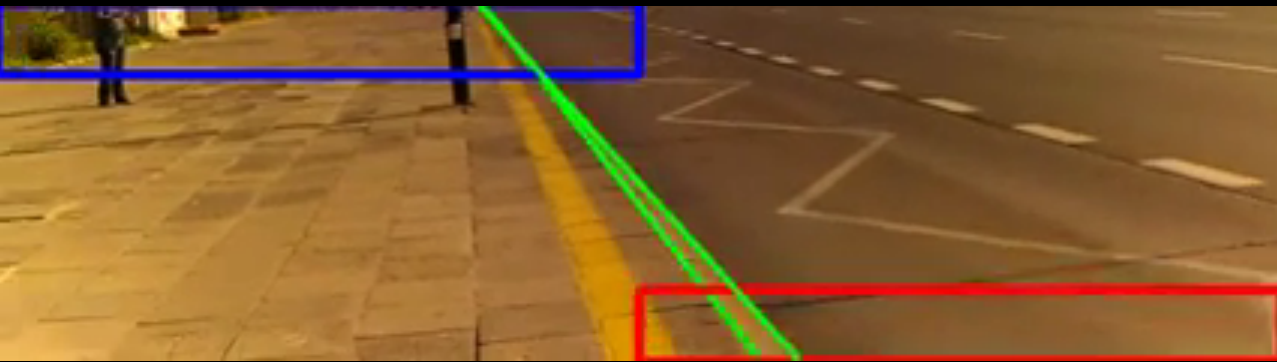
\includegraphics[width=0.9\textwidth]{img/exp_bus_lane_edge_detector}
    \caption{Wykrywacz linii krawędzi zatoki autobusowej}
    \label{fig:bus_lane_edge_detection}
\end{figure}

Rysunek \ref{fig:bus_lane_edge_detection} przedstawia wynik 
eksperymentalnej wersji programu do
wykrywania krawędzi zatoki autobusowej. W~implementacji użyty
został prosty ,,Canny edge detector''. Zakładając, że osoba stojąca
na przystanku jest skierowana twarzą (kamerą) do nadjeżdżającego autobusu,
linia wyznaczona przez krawężnik zatoki powinna zaczynać się w~połowie
wysokości klatki (obraz na powyższym rysunku przedstawia jej dolną
połowę) bardziej z~lewej strony - niebieski prostokąt. Koniec linii
powinien znajdować się na dole klatki bardziej z~prawej strony - czerwony
prostokąt.

Zrezygnowano z~tego pomysłu ze względu na zbyt dużą ilość 
specyficznych
ograniczeń geometrycznych i~niezamierzoną dyskryminację pasażerów
których zatoki przystankowe nie mają krawężników. Ostatnim argumentem
na niekorzyść, 
byli inni pasażerowie stojący na przystanku, którzy najzwyczajniej
zasłaniali krawężnik na przystanku czyniąc metodę tę bezużyteczną.

Na tym etapie podjęta została decyzja, że wstępna segmentacja
zostanie wykonana przy użyciu kaskadowego detektora cech (HAAR, HOG, LBP)
opisana w~artykule, które autorami byli panowie Viola i~Jones.

\subsection{Progowanie HSV}

Równoległym pomysłem do kaskadowego detektora było 
wykorzystanie progowania obrazu w~dziedzinie HSV (\textit{
ang. Hue Saturation Value})
w~celu wyodrębnienia wyświetlacza z~numerem linii. 
Kolejne niepokojące założenie, które poczyniono
na wstępnym etapie prac dotyczyło koloru numeru linii autobusowej.
Przyjęto, że odcień numeru będzie (w~znacznej ilości przypadków) 
zbliżony do pomarańczowego - z~możliwością rozszerzenia o~kolor
zielony. 

\begin{figure}[h!]
    \centering
    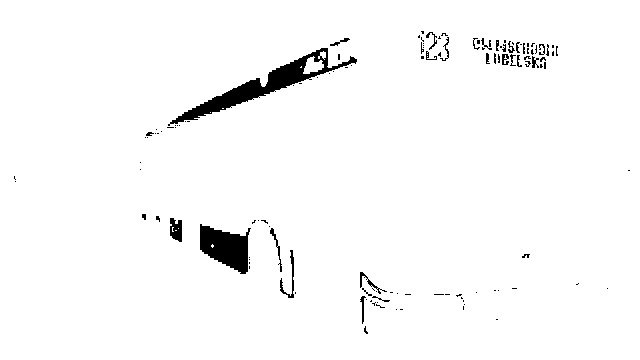
\includegraphics[width=0.9\textwidth]{img/exp_hsv_threshold_number_detector}
    \caption{Segmentacja numeru metodą progowania HSV}
\end{figure}

Po wykryciu potencjalnego numeru należałoby uruchomić drugi stopień
kaskady, który stwierdzałby czy dany fragment rzeczywiście reprezentuje
numer.

Niestety niepewność związana z~niepożądanym wykrywaniem przypadkowych
pomarańczowych numerów i~dyskryminacją pasażerów, którzy
poruszają się autobusami z~zielonymi wyświetlaczami skutecznie
zniechęciła do implementacji rzeczonego rozwiązania.

Na tym etapie dodatkowym argumentem było niepożądane 
pominięcie w~ten sposób
wszystkich autobusów z~tabliczkami gdzie numer zapisywany jest czarną
czcionką na białym tle. Argument ten był jeszcze wtedy aktualny, choć
ostatecznie zrezygnowano z~wykrywania frontów tzw. ,,starego typu'' -
Ikarus, Jelcz Berliet itp. Zostało to pośrednio wymuszone przez 
znacznie mniejszą skuteczność uniwersalnego detektora, który był
wyszkolony przy użyciu frontów z~tabliczkami i~tych z~wyświetlaczami, 
o~czym szerzej w~jednym z~następnych podrozdziałów.

\subsection{Gotowy silnik OCR - Tesseract}

Pierwsza próba z~narzędziem Tesseract okazała się bardzo obiecująca.
Ręcznie wycięty fragment reprezentujący numer 140 został podany 
jako argument wywołania komendy \verb|tesseract|:

\lstinputlisting{data/tesseractcommand.txt}

Parametr \verb|-psm 8| określał metodę segmentacji obrazu jako ,,jedno
słowo''. Obraz wejściowy \verb|nuber.png| został zaprezentowany
na rysunku \ref{fig:sample_tesseract_input}. Wynik jaki otrzymano dla 
powyższego doświadczenia
był wzorowy - w~pliku wynikowym \verb|out.txt| pojawił
się oczekiwany ciąg znaków (140).

\begin{figure}[h!]
    \centering
    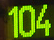
\includegraphics[width=0.25\textwidth]{img/exp_number_01}
    \caption{Pierwszy numer testowy - prawidłowo odczytany}
    \label{fig:sample_tesseract_input}
\end{figure}

Szereg kolejnych doświadczeń przyniósł jednak rozczarowanie. 
Wiele dobrze widocznych numerów w~stosunkowo wysokiej rozdzielczości 
nie zostało odczytanych w~ogóle (ciąg znaków zerowej długości). Zdarzały 
się nawet przypadki kiedy trzycyfrowy numer został rozszyfrowany jako
kilka wielocyfrowych liczb (ciąg ze spacjami).

\begin{table}[h!]
  \centering
  \begin{tabular}{c l c l c l}
    Obraz1 & Odczyt1 & Obraz2 & Odczyt2 & Obraz3 & Odczyt3  \\ 
    \begin{minipage}{.2\textwidth}
      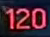
\includegraphics[width=\textwidth]{img/exp_number_02}
    \end{minipage}
    &
    120
    &
    \begin{minipage}{.2\textwidth}
      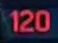
\includegraphics[width=\textwidth]{img/exp_number_03}
    \end{minipage}
    &
    120.
    &
    \begin{minipage}{.2\textwidth}
      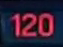
\includegraphics[width=\textwidth]{img/exp_number_04}
    \end{minipage}
    &
    120
    \\
    \begin{minipage}{.2\textwidth}
      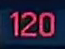
\includegraphics[width=\textwidth]{img/exp_number_05}
    \end{minipage}
    &
    120
    &
    \begin{minipage}{.2\textwidth}
      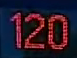
\includegraphics[width=\textwidth]{img/exp_number_06}
    \end{minipage}
    &
    120
    &
    \begin{minipage}{.2\textwidth}
      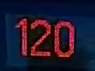
\includegraphics[width=\textwidth]{img/exp_number_07}
    \end{minipage}
    &
    120
    \\ 
  \end{tabular}
  \caption{Wyniki pierwszej serii testowej tesseract}\label{tbl:tess_01}
\end{table}

Niestety w~momencie pisania tego tekstu wyniki pierwotnych eksperymentów
zostały utracone. Mając już gotową implementacją opartą na innym
rozwiązaniu wykonano dwie krótkie serie próbne, których wyniki
zamieszczono w~tabelkach poniżej.

Pierwsza seria próbna pokazuje, że rozwiązanie oparte na narzędziu
Tesseract ma duży potencjał i~wysokie prawdopodobieństwo powodzenia.
Jednak aby zobrazować problemy jakie niesie ze sobą to podejście
wykonano dwie kolejne, celowo nieudane próby.

\begin{table}[h!]
  \centering
  \begin{tabular}{c l c l}
    Obraz1 & Odczyt1 & Obraz2 & Odczyt2  \\ 
    \begin{minipage}{.2\textwidth}
      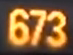
\includegraphics[width=\textwidth]{img/exp_number_n01}
    \end{minipage}
    &
    673
    &
    \begin{minipage}{.2\textwidth}
      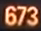
\includegraphics[width=\textwidth]{img/exp_number_n02}
    \end{minipage}
    &
    673
     
    \\ 

    \begin{minipage}{.2\textwidth}
      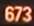
\includegraphics[width=\textwidth]{img/exp_number_n03}
    \end{minipage}
    &
    673
    &
    \begin{minipage}{.2\textwidth}
      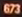
\includegraphics[width=\textwidth]{img/exp_number_n04}
    \end{minipage}
    &
    .

    \\ 

  \end{tabular}
  \caption{Wyniki drugiej serii testowej tesseract}\label{tbl:tess_02}
\end{table}

W~drugiej serii przedstawiono zależność skuteczności Tesseracta od 
rozdzielczości obrazu, gdzie czwarty obraz został zinterpretowany
jako kropka. Poziom dokładności jest w~tym przypadku na poziomie
jak najbardziej akceptowalnym. Trudno nawet spodziewać się lepszego
wyniku.

Największe wątpliwości
co do wykorzystania Tesseracta w~rozwiązaniu docelowym zostały zobrazowane
przez wyniki trzeciej serii testowej. Tutaj zniekształcenia spowodowane
refleksami pojawiającymi się na szybie osłaniającej wyświetlacz
zupełnie uniemożliwiły skuteczne odczytanie numeru.

\begin{table}[h!]
  \centering
  \begin{tabular}{c l c l c l}
    Obraz1 & Odczyt1 & Obraz2 & Odczyt2 & Obraz3 & Odczyt3  \\ 
    \begin{minipage}{.2\textwidth}
      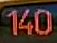
\includegraphics[width=\textwidth]{img/exp_number_f01}
    \end{minipage}
    &
     26
    &
    \begin{minipage}{.2\textwidth}
      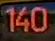
\includegraphics[width=\textwidth]{img/exp_number_f02}
    \end{minipage}
    &
    170
    &
    \begin{minipage}{.2\textwidth}
      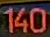
\includegraphics[width=\textwidth]{img/exp_number_f03}
    \end{minipage}
    &
    140
    \\
    \begin{minipage}{.2\textwidth}
      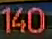
\includegraphics[width=\textwidth]{img/exp_number_f04}
    \end{minipage}
    &
     9.
    &
    \begin{minipage}{.2\textwidth}
      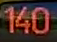
\includegraphics[width=\textwidth]{img/exp_number_f05}
    \end{minipage}
    &
    
    &
    \begin{minipage}{.2\textwidth}
      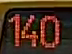
\includegraphics[width=\textwidth]{img/exp_number_f06}
    \end{minipage}
    &
    
    \\
    \begin{minipage}{.2\textwidth}
      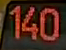
\includegraphics[width=\textwidth]{img/exp_number_f07}
    \end{minipage}
    &
     1420.
    &
    \begin{minipage}{.2\textwidth}
      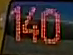
\includegraphics[width=\textwidth]{img/exp_number_f08}
    \end{minipage}
    &
     711913
    &

  \end{tabular}
  \caption{Wyniki trzeciej serii testowej tesseract}\label{tbl:tess_03}
\end{table}

Dodatkowym problemem jest prawdopodobna tendencja do nadinterpretacji
przy odczycie numerów gdy rozdzielczość jest już na tyle wysoka, że
widoczne są poszczególne diody - ostatni obraz z~serii trzeciej.
Rozwiązaniem tego problemu byłoby zastosowanie adaptacyjnego filtru
Gaussa lub operacji morfologicznych, np.: otwarcia + zamknięcia.
Opór przed tego typu zabiegami spowodowany brakiem narzędzi 
do mierzenia skuteczności zaowocował pominięciem narzędzi Tesseract
w~rozwiązaniu końcowym. Tym nie mniej jest to metoda z~największym
potencjałem spośród omawianych do tej pory ,,ślepych uliczek''. 
Fakt, że w~trzech powyższych próbach dwie z~nich dały wynik pozytywny
i~to bez wcześniejszej konfiguracji narzędzia (nauka dodatkowych
krojów czcionek itp.) świadczy, że można z~powodzeniem próbować
usprawnić proponowane w~tym opracowaniu rozwiązanie poprzez 
podmianę ostatniego (czwartego) kroku kaskady w~oparciu o~narzędzie
Tesseract. Tym bardziej, że wspomniany program posiada gotową
implementację działającą na systemie Android.

\subsection{MSER - lokalizacja numeru}

Ostatnim eksperymentem, którego wyniki nie były dostatecznie przekonujące
do użycia badanej metody w~rozwiązaniu docelowym, było
wykorzystanie algorytmu MSER (\textit{ang. Most Stable Extreme Regions})
do określania położenia numeru.

\begin{figure}[h!]
    \centering
    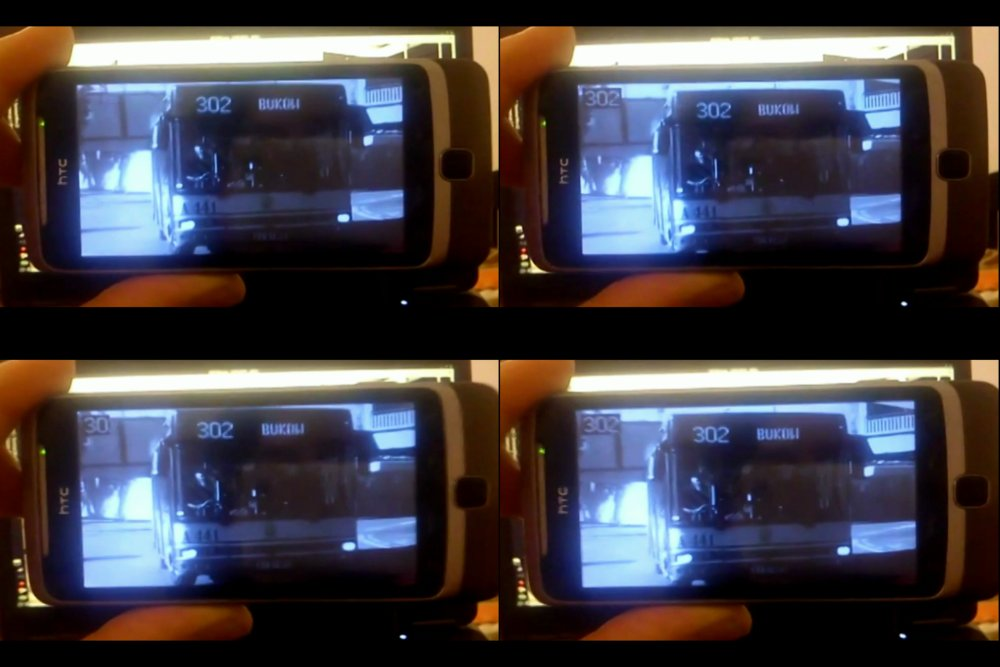
\includegraphics[width=0.9\textwidth]{img/exp_mser_concerns}
    \caption{Pierwszy numer testowy - prawidłowo odczytany}
    \label{fig:mser_example_results}
\end{figure}

Poglądowe rezultaty zostały zaprezentowane na rysunku
\ref{fig:mser_example_results}.
Niestety w~zależności od rozdzielczości zmieniała się podatność
numeru na wykrycie. Dla niewielkich rozdzielczości numer był rozpoznawany
jedynie jako całość, gdzie ograniczeniem geometrycznym wykorzystanym
do tego celu był prostokąt pocztówkowy o~proporcjach 2 na 3 - prezentowany
przykład. Na lewym dolnym obrazie można zaobserwować wykrycie jedynie
pierwszych dwóch cyfr numeru.

W~wyższych rozdzielczościach aby zachować wprowadzone ograniczenie
niezbędne było zastosowanie filtru rozmywającego. Bez filtru
wykrywane regiony reprezentowały poszczególne cyfry składowe numeru.
W~tym przypadku ograniczenie geometryczne wahało się od 1x4 (pionowy
prostokąt) dla jedynki do 2x3 (również prostokąt ustawiony pionowo) dla
pozostałych cyfr.

Zbyt duża liczba czynników wpływających na skuteczność:

\begin{itemize}
    \item krój czcionki: wysokie, wąskie,
    \item inne ograniczenia geometryczne dla zmiennej ilości cyfr
        w~numerze,
    \item stosowanie adaptacyjnych filtrów celem rozmycia obrazów
        w~wyższych rozdzielczościach (autobus bliżej obserwatora),
    \item stosowanie dwóch niezależnych detektorów, oddzielnie dla
        cyfr i~oddzielnie dla numerów.
\end{itemize}

spowodowały, że pominięto tę metodę w~rozwiązaniu końcowym.
Tym nie mniej jest to druga (po narzędziu tesseract) metoda, której
wyniki były na tyle obiecujące, że przemyślana implementacja
mogłaby z~powodzeniem zastąpić ostatecznie wykorzystany kaskadowy
detektor oparty na cechach Haara.


\section{Eksperymentu częściowo udane - pierwsza iteracja}

W~podrozdziale tym przedstawione i~omówione zostały doświadczenia
związane z~algorytmami, narzędziami i~bibliotekami wykorzystanymi
w~ostatecznym programie
(pierwszej wersji testowej). Opis powstawał równolegle
do toczących się prac więc wykazuje pewne cechy sprawozdania
lub relacji na bieżąco.
Prezentacja oraz dokładna analiza wyników powstała w~drugiej
iteracji, kiedy to godowy był już działający prototyp.
Druga tura miała na celu rzetelną weryfikację skuteczności
i~wydajności drugiej wersji programu (tzw. wersji beta).

W~ramach pierwszej iteracji
wprowadzony został logiczny podział na pięć etapów:

\begin{enumerate}
    \item Przygotowanie zbioru uczącego (który miał być jednocześnie
        zbiorem testowym). Początkowo przyjęta forma przechowywania danych
        - pełne klatki w~których oznaczone były wystąpienia
        frontów oraz osobny plik tekstowy ze współrzędnymi -
        pozwalała na wykorzystanie zbioru uczącego również
        w~procesach testowych. 
        Próba ograniczenia miejsca zajmowanego przez zbiór -
        przechowywanie wycinków
        zawierających tylko szukane obiekty - 
        uniemożliwiło wykorzystanie zbioru uczącego podczas 
        testów. Funkcja
        gorzej radziła sobie z~wyszukiwaniem obiektów, które nie
        zawierały dostatecznego marginesu wokół obiektów.
        Był to jeden z~powodów przeprowadzenia drugiej iteracji
        w~procesie przygotowywania programu końcowego.
    \item Wstępna segmentacja - wyszukiwanie frontu autobusu, wraz
        z~dodatkową analizą wpływu zadanych parametrów na skuteczność
        szkolonego detektora.
    \item Wyłuskanie fragmentu obrazu zawierającego wyłącznie numer -
        kaskadowy detektor wykrywający numery.
    \item Dziesięć detektorów wykrywających cyfry i~ich wykorzystanie
        w~celu zawężenia obszaru poszukiwań w~procesie dopasowywania 
        wzorca (\textit{ang. Template Matching}), który to proces
        jest najbardziej intensywny obliczeniowo z~użytych.
        W~drugiej wersji krok ten rozbito na dwa:
        \begin{itemize}
            \item wyszukiwanie cyfr we fragmencie reprezentującym numer
                za pomocą pojedynczego detektora dla wszystkich cyfr,
            \item rozpoznawanie zidentyfikowanych fragmentów na
                podstawie wektora cech podanego na klasyfikator SVM.
        \end{itemize}
    \item Krótkie testy związane ze skutecznością i~zasadnością
        wykorzystania metody \textit{Template Matching} w~celu weryfikacji
        potencjalnych obszarów reprezentujących cyfry.
\end{enumerate}

Pierwszy etap pochłonął najwięcej czasu. Podjęte zostały próby 
przygotowania procedury i~oprogramowania wspomagających określenie
skuteczności implementowanych rozwiązań oraz określenia 
najbardziej optymalnych parametrów do wykorzystania podczas procesu
uczenia detektora narzędziem z~pakietu OpenCV: \verb|train_cascade|.

O~ile skuteczność znajdowania frontów autobusów - wstępna segmentacja - 
jest kluczowa dla poprawnego funkcjonowania projektowanego programu 
i~zasadnym jest jej rzetelne przetestowanie to skuteczność pozostałych
etapów - ze względu na zastosowane ograniczenia - nie jest już tak
istotna (o~czym więcej w~następnym rozdziale). Pewnym usprawiedliwieniem
i~w~pewnym sensie powodem nie przetestowania wszystkich parametrów
wejściowych narzędzia do szkolenia detektorów był czas ich szkolenia 
- od jednej do kilkunastu godzin, dla detektora cech LBP. Ostatecznie
celem nie była analiza samych narzędzi a~opracowanie i~implementacja
skutecznego programu do odczytywania numerów nadjeżdżających autobusów.

\subsection{Zbiór danych uczących i testowych}

Dane wykorzystane do procesu uczenia detektorów frontów autobusów
składały się z~dwóch części.
Pierwszą partią danych było 11 zestawów obrazów
przygotowanych z~uprzednio pobranych filmów z~serwisu YouTube.
Każdy zestaw składał się z co najmniej dwóch zbiorów. Obrazów 
reprezentujących oznaczone fronty autobusów oraz obrazów tła. 
Opcjonalnym zbiorem był zestaw oznaczonych 
frontów autobusów typu Solaris. Osobny zestaw frontów miał na celu
porównanie skuteczności detektorów przygotowanych tylko przy pomocy
pojedynczego typu obiektu oraz tych do przygotowania których użyto
obiektów znacząco od siebie różnych.

Drugi zestaw (oznaczony ponownie w~ramach drugiej iteracji) 
to obrazy pobrane z~serwisu \verb|http://www.phototrans.eu/|.
Zbiór ten zawierał 9067 kwadratowych wycinków różnych rozmiarów
przedstawiających wyłącznie fronty autobusów. Ze względu na mnogość
typów i~nieusystematyzowanie zbioru jego szczegółowy opis nie będzie
zamieszczony. Ze względu na specyfikę skryptu pobierającego zdjęcia
z~serwisu zostały ułożone zgodnie z~kolejnością linii autobusowych.
Kolejność jest pseudo alfabetyczna, gdzie w~pierwszej kolejności
są numery jednocyfrowe, potem kolejno dwu i~trzycyfrowe.

Poniżej zamieszczono szczegółowy opis części pierwszej zbioru.
Podział na autobusy Solaris i Inne okazał się nietrafiony. 
W~naturalny sposób podczas uczenia detektorów zidentyfikowany został 
inny podział o~czym w~kolejnych rozdziałach.

\subsubsection{Zbiór jJ9ixBfVR5k}

W~zbiorze znalazły się następujące typy autobusów: 
\begin{itemize}
    \item Jelcz: M121M (x:3,y:1), M121CNG (x:4,y:1),
    \item Ikarus 280 (x:1, y:1),
    \item Man: NL223 (x:2, y:[1:2]), (x:3, y:2 - zielony wyświetlacz),
        Lion's City (x:4, y:2),
    \item Scania OmniCity CN (x:1, y:2). 
\end{itemize}
Współrzędne w~nawiasach określają pozycję modelu autobusu na rysunku
\ref{fig:jJ9ixBfVR5k_types}.
Jeden z modeli autobusów Man został wyposażony w zielony wyświetlacz numeru.
Jest to bardzo trudny przypadek w kontekście rozpoznawania numeru.

\begin{figure}[!h]
    \centering
    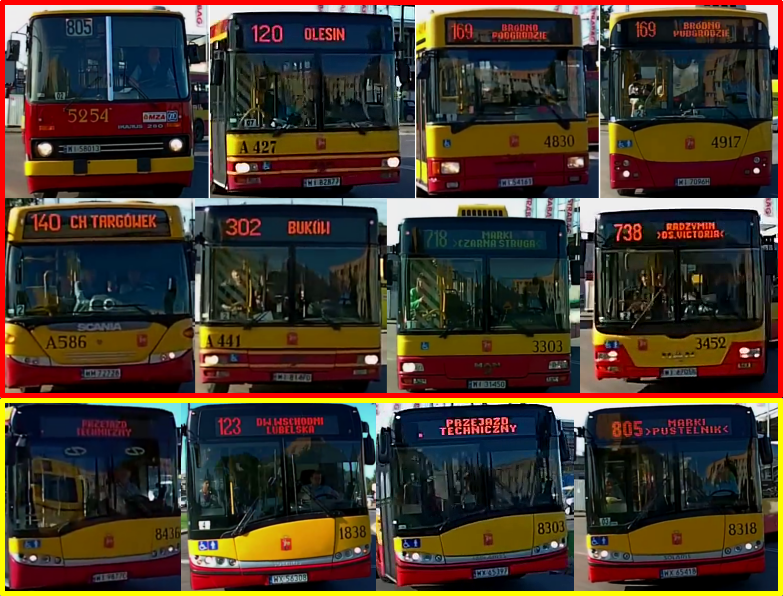
\includegraphics[width=0.8\textwidth]{img/exp_trainig_data_jJ9}
    \caption{Typy autobusów zawarte w zbiorze jJ9ixBfVR5k}
    \label{fig:jJ9ixBfVR5k_types}
\end{figure}

Liczebność zebranych próbek została przedstawiona w~tabelce nr. 
\ref{tab:jJ9ixBfVR5k_count}.

\begin{table}[!h]
    \centering
    \begin{tabular}{c|c|c}
        Front   & Solaris   & Background \\ \hline
        2587    & 222       & 2239
    \end{tabular}
    \caption{Liczebność zbioru jJ9ixBfVR5k}
    \label{tab:jJ9ixBfVR5k_count}
\end{table}

\subsubsection{Zbiór vYqZ4-tH4M0}

W~zbiorze znalazły się te same dwa modele autobusu Jelcz co w~zbiorze
poprzednim. Powtórzyły się także modele: Ikarus, Scania oraz dwa modele
autobusów Man. Dodatkowo pojawił się model: Mercedes Citaro, oraz trzy 
niezidentyfikowane bliżej modele - pozycje: druga, trzecia i~czwarta 
w~rzędzie drugim na rysunku \ref{fig:vYqZ4-tH4M0_types} 
(prawdopodobnie Solaris, Autosan oraz Jelcz).

\begin{figure}[!h]
    \centering
    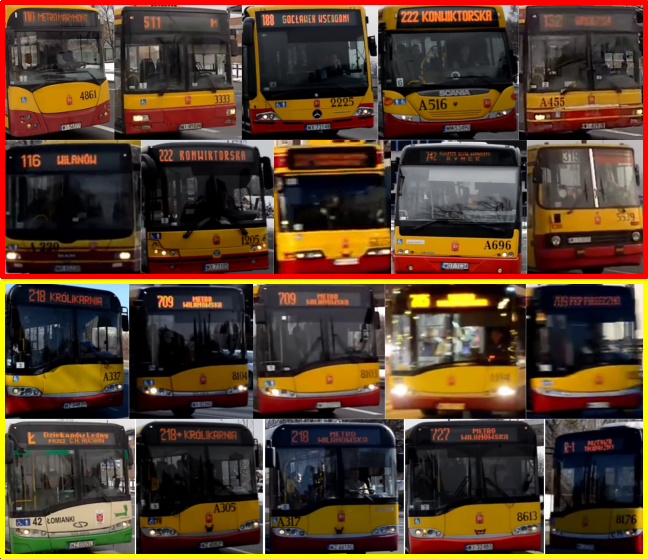
\includegraphics[width=0.9\textwidth]{img/exp_trainig_data_vYq}
    \caption{Typy autobusów zawarte w zbiorze vYqZ4-tH4M0}
    \label{fig:vYqZ4-tH4M0_types}
\end{figure}

Jeżeli chodzi o~liczebność to podzbiór ten plasuje się w~środku 
zestawienia.
Dokładne dane zamieszczono w~tabeli \ref{tab:vYqZ4-tH4M0_count}.

\begin{table}[!h]
    \centering
    \begin{tabular}{c|c|c}
        Front   & Solaris   & Background \\ \hline
        291     & 320       & 230 
    \end{tabular}
    \caption{Liczebność zbioru vYqZ4-tH4M0}
    \label{tab:vYqZ4-tH4M0_count}
\end{table}

\newpage

\subsubsection{Zbiór J8h8j6096Uw}

W~zbiorze zabrakło zdjąć reprezentujących fronty autobusów marki
Solaris. Znalazły się natomiast dwa modele marki Man - wersja 
z~,,płaską'' maską (NL223) oraz model z~charakterystycznym czarnym
wgłębieniem w~centralnej jej części (Lion's City).

\begin{figure}[!h]
    \centering
    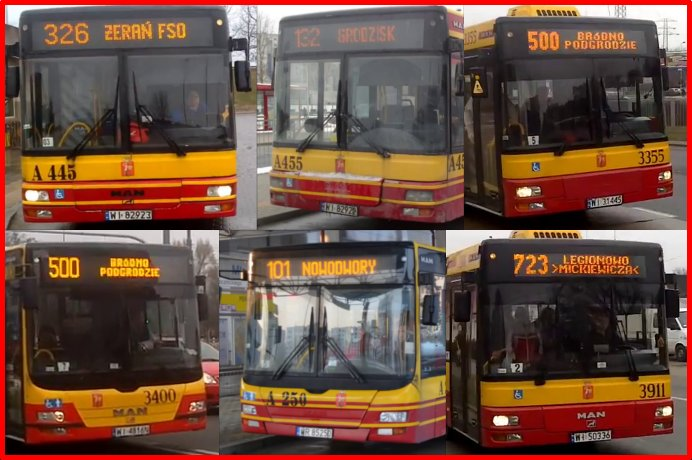
\includegraphics[width=0.65\textwidth]{img/exp_trainig_data_J8h}
    \caption{Typy autobusów zawarte w zbiorze J8h8j6096Uw}
    \label{fig:J8h8j6096Uw_types}
\end{figure}

\begin{table}[!h]
    \centering
    \begin{tabular}{c|c|c}
        Front   & Solaris   & Background \\ \hline
        182     & brak      & 427 
    \end{tabular}
    \caption{Liczebność zbioru J8h8j6096Uw}
    \label{tab:J8h8j6096Uw_count}
\end{table}

\subsubsection{Zbiór aO71uxrP9B0}

W~zbiorze miejsce znalazły zaledwie dwa modele autobusu Volvo oraz
występujący już wcześniej Mercedes Citaro.

\begin{figure}[!h]
    \centering
    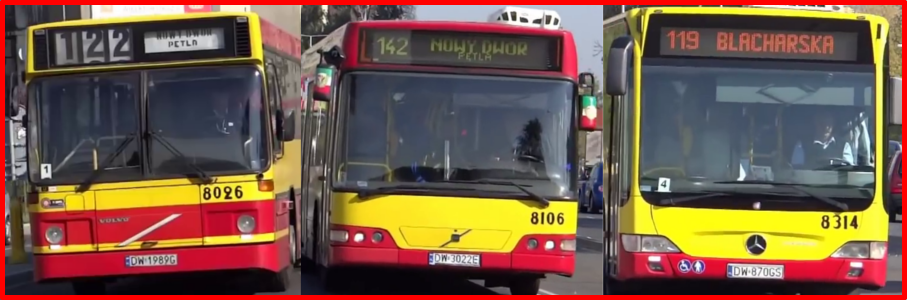
\includegraphics[width=0.65\textwidth]{img/exp_trainig_data_aO7}
    \caption{Typy autobusów zawarte w zbiorze aO71uxrP9B0}
    \label{fig:aO71uxrP9B0_types}
\end{figure}

\begin{table}[!h]
    \centering
    \begin{tabular}{c|c|c}
        Front   & Solaris   & Background \\ \hline
        177     & brak      & 977 
    \end{tabular}
    \caption{Liczebność zbioru aO71uxrP9B0}
    \label{tab:aO71uxrP9B0_count}
\end{table}

\newpage

\subsubsection{Zbiór J6sD0Tc2Dbs}

Zbiór ten zawiera dwa rodzaje autobusów marki Man oraz dwie wersje autobusu
Solaris - ze znaczkiem na masce oraz bez niego (maska gładka). Wyświetlacze
prezentujące numer wykorzystane w~przedstawionych modelach Solarisów
skutecznie uniemożliwiają odczytanie go przez jakiekolwiek urządzenie. 
Nawet człowiek nie jest w~stanie domyślić się numeru który został utrwalony
na zdjęciach - rysunek \ref{fig:J6sD0Tc2Dbs_types}. Historyczne modele
skody zostały zaprezentowane w~ramach ciekawostki i~nie będą uwzględniane
w~dalszych eksperymentach.

\begin{figure}[!h]
    \centering
    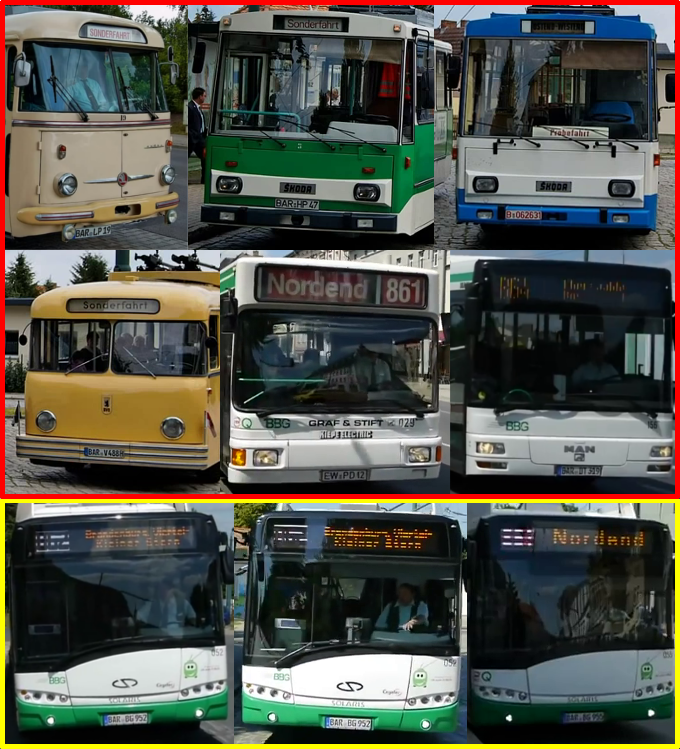
\includegraphics[width=0.65\textwidth]{img/exp_trainig_data_J6s}
    \caption{Typy autobusów zawarte w zbiorze J6sD0Tc2Dbs}
    \label{fig:J6sD0Tc2Dbs_types}
\end{figure}

\begin{table}[!h]
    \centering
    \begin{tabular}{c|c|c}
        Front   & Solaris   & Background \\ \hline
        156     & 124       & 203 
    \end{tabular}
    \caption{Liczebność zbioru J6sD0Tc2Dbs}
    \label{tab:J6sD0Tc2Dbs_count}
\end{table}

\newpage

\subsubsection{Zbiór IHarVPkXwSg}

W~zbiorze - podobnie jak poprzednio - znalazły się autobusy zabytkowe.
Modele w~rzędzie pierwszym (dotyczy pozycji pierwszej i~drugiej) nie 
będą wykorzystane w~dalszych eksperymentach. Mają na celu uzmysłowienie
stopnia złożoności problemu oraz fakt, że w~zależności od modelu pozycja
numeru może oscylować w~ramach górnej połowy obszaru zidentyfikowanego
jako front autobusu. Pozostałe modele, czyli
dwa modele Jelcza, Mercedes i~(prawdopodobnie, jakiś) model Mana tworzą
grupę frontów ,,różnych''. W~skład zbioru wchodzą też dwa typy autobusu
solaris - różne kształty maski.

\begin{figure}[!h]
    \centering
    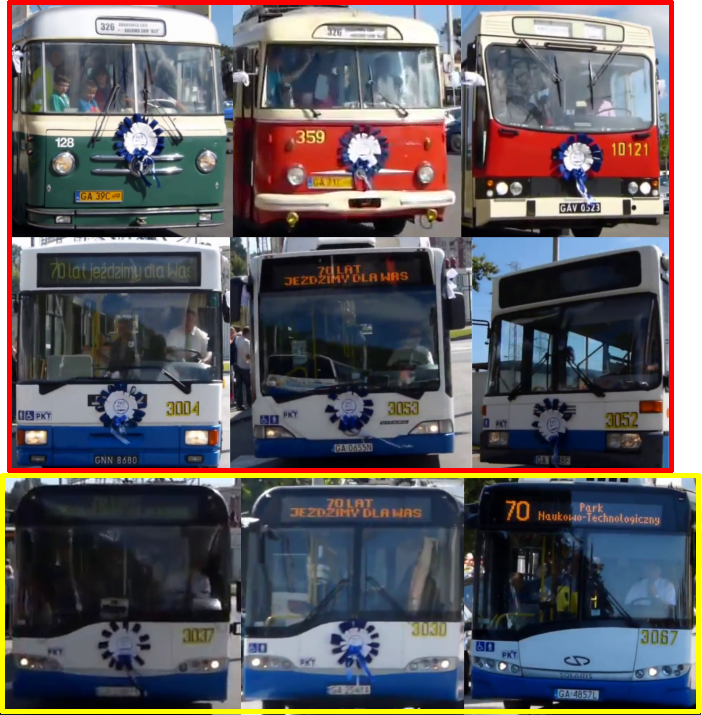
\includegraphics[width=0.8\textwidth]{img/exp_trainig_data_IHa}
    \caption{Typy autobusów zawarte w zbiorze IHarVPkXwSg}
    \label{fig:IHarVPkXwSg_types}
\end{figure}

\begin{table}[!h]
    \centering
    \begin{tabular}{c|c|c}
        Front   & Solaris   & Background \\ \hline
        342     & 172       & 1510
    \end{tabular}
    \caption{Liczebność zbioru IHarVPkXwSg}
    \label{tab:IHarVPkXwSg_count}
\end{table}

\subsubsection{Zbiór BJZLDmYMFvo}

Zbiór zawiera jedynie dwa modele autobusu Man, oraz autobusy marek
Jelcz i Solaris. Jedyna uwaga może tyczyć trudności w~odczytywaniu
numeru z~autobusu man/jelcz z~wyświetlaczem w~kolorze zielonym. Jeżeli tylko
warunki oświetleniowe są dobre - jak na rysunku \ref{fig:BJZLDmYMFvo_types}
- widoczność, a~co za tym idzie rozpoznawalność numeru powinna być na 
zadowalającym poziomie.

\begin{figure}[!h]
    \centering
    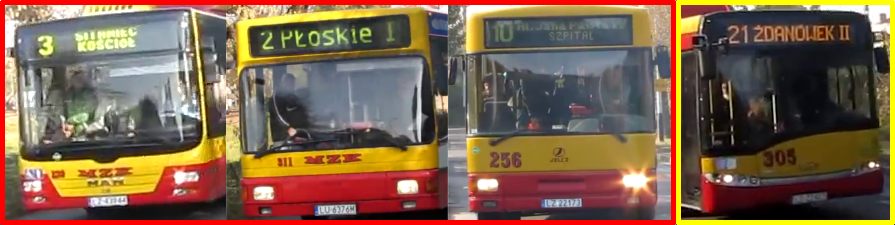
\includegraphics[width=0.95\textwidth]{img/exp_trainig_data_BJZ}
    \caption{Typy autobusów zawarte w zbiorze BJZLDmYMFvo}
    \label{fig:BJZLDmYMFvo_types}
\end{figure}

Zbiór ten posiada drugą co do wielkości 
liczbę obrazów tła (w~pierwszej iteracji). 

\begin{table}[!h]
    \centering
    \begin{tabular}{c|c|c}
        Front   & Solaris   & Background \\ \hline
        373     & 8         & 2356
    \end{tabular}
    \caption{Liczebność zbioru BJZLDmYMFvo}
    \label{tab:BJZLDmYMFvo_count}
\end{table}

\subsubsection{Zbiór \_43HUVkrA7E}

Zbiór składający się głównie ze zdjęć zawierających oznaczone fronty
zabytkowego już autobusu Jelcz Berliet. Jeżeli chodzi o~liczebność to 
główną wartością dodaną są obrazy reprezentujące tło.

\begin{figure}[!h]
    \centering
    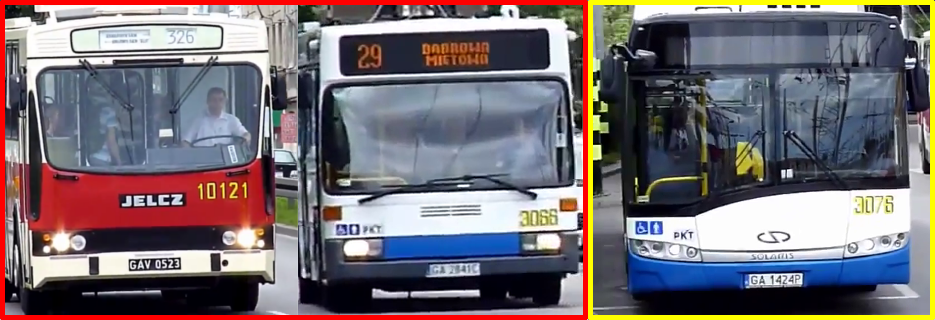
\includegraphics[width=0.75\textwidth]{img/exp_trainig_data__43}
    \caption{Typy autobusów zawarte w zbiorze \_43HUVkrA7E}
    \label{fig:_43HUVkrA7E_types}
\end{figure}

\begin{table}[!h]
    \centering
    \begin{tabular}{c|c|c}
        Front   & Solaris   & Background \\ \hline
        44      & 5         & 197 
    \end{tabular}
    \caption{Liczebność zbioru \_43HUVkrA7E}
    \label{tab:_43HUVkrA7E_count}
\end{table}

\subsubsection{Zbiór 8wdvLn40CTk}

Najmniejszy zbiór w~kontekście różnorodności zawartych modeli. Z~drugiej
strony ogromna ilość obrazów tła oraz relatywnie dużo oznaczonych ujęć.

\begin{figure}[!h]
    \centering
    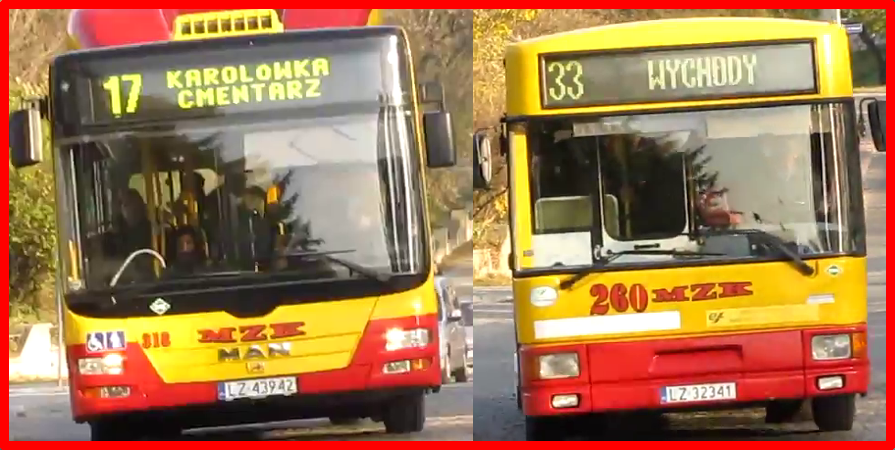
\includegraphics[width=0.45\textwidth]{img/exp_trainig_data_8wd}
    \caption{Typy autobusów zawarte w zbiorze 8wdvLn40CTk}
    \label{fig:8wdvLn40CTk_types}
\end{figure}

\begin{table}[!h]
    \centering
    \begin{tabular}{c|c|c}
        Front   & Solaris   & Background \\ \hline
        336     & brak      & 3572
    \end{tabular}
    \caption{Liczebność zbioru 8wdvLn40CTk}
    \label{tab:8wdvLn40CTk_count}
\end{table}

\subsubsection{Zbiór 75Dz6s7S-Tg}

Kolejny niewielki zbiór. Te same modele autobusu Man co w~zestawie
pierwszym. Dodatkowo dwie wersje kolorystyczne (wyświetlacz) modelu
Mercedes Citaro. Na koniec wystąpienie modelu Solaris niestety zaledwie
w~dwóch egzęplażach.

\begin{figure}[!h]
    \centering
    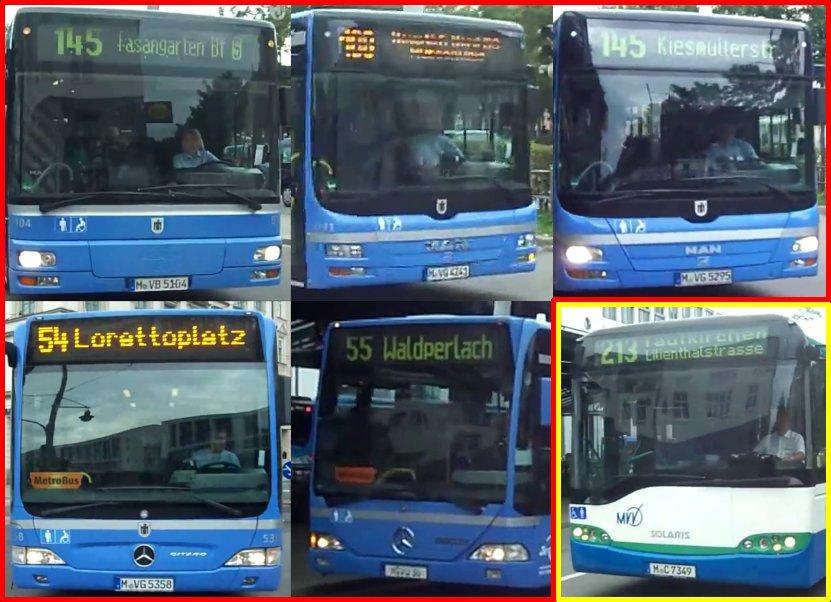
\includegraphics[width=0.75\textwidth]{img/exp_trainig_data_75D}
    \caption{Typy autobusów zawarte w zbiorze 75Dz6s7S-Tg}
    \label{fig:75Dz6s7S-Tg_types}
\end{figure}

\begin{table}[!h]
    \centering
    \begin{tabular}{c|c|c}
        Front   & Solaris   & Background \\ \hline
        81      & 2         & 179 
    \end{tabular}
    \caption{Liczebność zbioru 75Dz6s7S-Tg}
    \label{tab:75Dz6s7S-Tg_count}
\end{table}

\subsubsection{Zbiór 9hMQ4UGNxhw}

Występujące już wcześniej modele: Mercedes Citaro, zabytkowy Jelcz Berliet,
Man Lion's City, Scania OmniCity, Ikarus 280 z~ledowym wyświetlaczem,
Jelcz M121CNG (x:2, y:1). Dodatkowo dwie wersje kolorystyczne autobusu
Autosan.

\begin{figure}[!h]
    \centering
    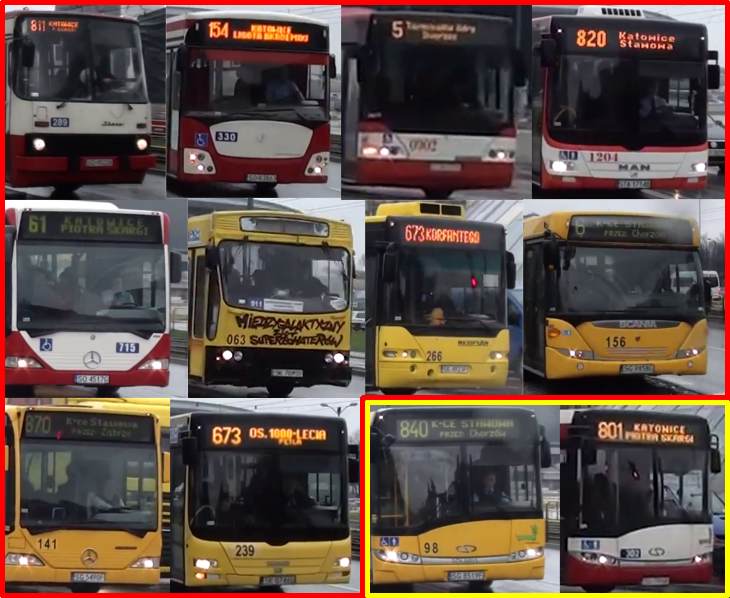
\includegraphics[width=0.95\textwidth]{img/exp_trainig_data_9hM}
    \caption{Typy autobusów zawarte w zbiorze 9hMQ4UGNxhw}
    \label{fig:9hMQ4UGNxhw_types}
\end{figure}

\begin{table}[!h]
    \centering
    \begin{tabular}{c|c|c}
        Front   & Solaris   & Background \\ \hline
        267     & 102       & 363 
    \end{tabular}
    \caption{Liczebność zbioru 9hMQ4UGNxhw}
    \label{tab:9hMQ4UGNxhw_count}
\end{table}

Ostatecznie po złączeniu wszystkich zaprezentowanych zbiorów powstały
dwa końcowe (będące jednocześnie punktem wyjścia do dalszych testów):
\begin{itemize}
    \item zbiór wszystkich oznaczonych frontów (różne + solarisy) 
        - 5781 sztuk,
    \item zbiór oznaczonych frontów autobusów typu Solaris - 955 sztuk.
\end{itemize}

Osobny zbiór zawierający tylko fronty typu Solaris miał na celu
sprawdzenie czy mnogość pozytywnych kształtów nie wpływa na skuteczność
detekcji. Stąd osobne dane uczące/testowe oraz detektor wykrywający 
tylko fronty typu Solaris. Jak się później okazało naturalny podział
- wykryty organoleptycznie, podczas oznaczania wystąpień frontów - 
wyznacza dwie grupy frontów: te z~wyświetlaczem led-owym (na całej
długości górnej krawędzi frontu) oraz te bez niego.

\subsection{Przygotowanie optymalnego detektora frontów}

Pierwsze próby związane z~procesem uczenia detektora miały na celu 
wyłonienie parametrów mających największy wpływ na skuteczność 
oraz efektywność trenowanego detektora.

\subsubsection{Porównanie detektorów HAAR, LBP i HOG}

Pierwsza iteracja uczenia detektorów miała na celu przetestowanie
opcji jakie można zadać narzędziu uczącemu \verb|opencv_traincascade|.

Za zbiór testowy posłużył zestaw oznaczonych zdjęć oraz zdjęć tła
przygotowany dla filmu o id jJ9ixBfVR5k (charakterystyka zbioru
została opisana w~poprzednim rozdziale)

Pierwszy test miał za zadanie wyłonić najefektywniejszą metodę, do dalszych
eksperymentów. Narzędzie dostarczone wraz z~pakietem OpenCV - wspomniany
już \verb|opencv_traincascade| - pozwalał na wyszkolenie trzech
rodzajów detektorów:

\begin{itemize}
    \item detektor wykorzystujący tzw. cechy Harra - wartość 
        domyślna (HAAR),
    \item detektor LBP,
    \item detektor HOG.
\end{itemize}

Gdy jeszcze nie wszystkie wyłuskane zdjęcia były opisane, wykonany został
krótki test porównawczy skuteczności i~czasu potrzebnego na nauczenie
poszczególnych typów detektorów. Po dość chaotycznie wykonanej próbie
otrzymano następujące wyniki:

\begin{table}[!h]
\centering
\begin{tabular}{r|c|c|c|l}
        & HAAR         & LBP        & HOG         & Wszystkie wystąpienia  \\
    \hline
Solaris & 151  (43\%)  & 81  (23\%) & 61 (17\%)   & 346  \\
Różne   & 1051 (35\%)  & 748 (25\%) & 712 (24\%)  & 2925 \\
Tło     & 635  (11\%)  & 386 (6\%)  & 447 (7\%)   & 5588 \\
\end{tabular}
\caption{Porównanie skuteczności detektorów typu HAAR, LBP i HOG.
Liczba poprawnie wykrytych frontów w~porównaniu do wszystkich opisanych
wystąpień.}
\label{tab:haar_lbp_hog_comparison}
\end{table}

Zaniżona wartość w~ostatniej wynikała z~faktu,
że nie wszystkie wyłuskane próbki były w~momencie wykonania testu opisane.
Łatwo jednak zaobserwować trend dokładności
tychże detektorów.

Kolejnym kryterium był czas uczenia detektorów.
O ile skuteczność detektora w~funkcji czasu potrzebnego na jego 
wyszkolenie dla detektorów cech HAAR-a i~LBP był skorelowany i~sensowny,
to w~przypadku cech HOG było już nieco inaczej.
Detektor oparty o~cechy HAAR-a potrzebował
zdecydowanie więcej czasu na wytrenowanie co miało przełożenie 
na jego skuteczność. LBP natomiast okazał się nieco mniej skuteczny
lecz jego szkolenie trwało krócej o~rząd wielkości.
Cechy HOG w~tym zestawieniu okazały się mało interesującym kandydatem
- skuteczność była gorsza niż LBP przy czasie szkolenie o~wiele dłuższym.

Czasy uczenia dla poszczególnych detektorów wyglądały następująco:
\begin{itemize}
    \item HAAR - 6 godzin
    \item HOG - 3 godziny
    \item LBP - 40 min
\end{itemize}

\subsubsection{Porównanie detektorów - Solaris i~frontów różnych}

Wbrew obawom detektor wyszkolony przy użyciu wszystkich 
rodzajów frontów 
wykazywał znacznie większą skuteczność podczas wykrywaniu 
frontów autobusów Solaris niż ten
wyszkolony z~użyciem tylko tego rodzaju frontów. Wyniki dla ustawień
domyślnych oraz detektora typu LBP przedstawiono w tabelce nr 
\ref{tab:sol_vs_all}. Znacznie większa skuteczność detektora
generycznego spowodowana jest zapewne przez efekt skali
gdzie detektor frontów różnych typów (w tym marki Solaris) 
był wyszkolony na kilkukrotnie większej liczbie próbek.

\begin{table}[!h]
    \centering
    \begin{tabular}{r|c|c|l}
          & Solaris    & Fronty różne   & Wszystkie wystąpienia (obrazy) \\
          \hline
wszystkie & 175 (3\%)  & 3466 (71\%)    & 4836      \\
solaris   & 609 (63\%) & 854 (89\%)     & 955       \\
błędy     & 289 (1\%)  & 56088 (310\%)  & 18048     \\
    \end{tabular}
    \caption{Skuteczność detektorów wyszkolonych tylko dla typów
    solaris w porównaniu do tych wyszkolonych dla wszystkich typów frontów
    (kolumny Solaris oraz Fronty różne)}
    \label{tab:sol_vs_all}
\end{table}

Jak widać problemem nie jest skuteczność wykrywania istniejących obiektów
tylko ogromna liczba wyników błędnych. W~kolejnych krokach zostaną opisane
próby poradzenia sobie z~tym problemem.

\subsubsection{Parametry minHitRate i~maxFalseAlarmRate}

W~celu przetestowania wpływu poszczególnych parametrów wejściowych
narzędzia do uczenia detektorów wykonano kilka sesji uczących 
przy zmiennych wartościach tychże parametrów. Pierwsza próba dotyczyła
parametrów:
\begin{itemize}
    \item minHitRate,
    \item maxFalseAlarmRate.
\end{itemize}
odpowiedzialnych za skuteczność wykrywania żądanych obiektów,
oraz podatność na błędne wykrycia.

Niestety wraz ze zwiększaniem parametru \verb|minHitRate|
znacząco zwiększała
się liczba błędnych trafień. Po wykonaniu pięciu sesji
uczących dla wartości parametru od 0.995 do 0.999 zaobserwowano 
ogromny wzrost błędnych trafień od odpowiednio 56 tysięcy
do 124 tysięcy (wykres \ref{chart:hitratio_fal}).

\begin{figure}[h!]
\begin{center}
\begin{tikzpicture}
\begin{axis}[
    ylabel={$Bledne\ trafienia$},
    xlabel={$minHitRate$},
    minor y tick num=1,
    width=\textwidth*0.6, height=5cm
]
\addplot [only marks, color=red] table {data/hitratio_fal.dat};
\end{axis}
\end{tikzpicture}
\end{center}
\caption{Zwiększenie liczby błędnych trafień przy zmianie parametru minHitRate}
\label{chart:hitratio_fal}
\end{figure}

W~stosunku do wielkiej liczby błędnych trafień procentowa skuteczność
wykrywania frontów autobusów rosła raczej w~sposób umiarkowany.


\begin{figure}[h!]
\begin{center}
\begin{tikzpicture}
\begin{axis}[
    ylabel={$Pozytywne\ trafienia$},
    xlabel={$minHitRate$},
    minor y tick num=1,
    yticklabel=\pgfmathprintnumber{\tick}\,\%,
    legend style={at={(0.06,0.73)},anchor=north west},
    width=\textwidth*0.6, height=6cm
]
\addplot [only marks, color=green] table {data/hitratio_fro.dat};
\addlegendentry{wszystkie}
\addplot [only marks, color=blue] table {data/hitratio_sol.dat};
\addlegendentry{solaris}
\end{axis}
\end{tikzpicture}
\end{center}
\caption{Zwiększenie liczby pozytywnych trafień przy zmianie parametru minHitRate}
\label{chart:hitratio_fro_sol}
\end{figure}

Pierwsza próba zmniejszenia nieudanych trafień polegała na zmianie 
parametru \verb|maxFalseAlarmRate| podczas uczenia detektora. 
Wykonano pięć
sesji uczenia detektora dla wartości: od domyślnej 0.5 do 0.1.

Ostatecznie przy ilości próbek pozytywnych i~negatywnych 
na poziomie 5000 opisywane wyżej parametry nie miały już prawie w~cale
znaczenia. Przy domyślnych wartościach skuteczność detektora była 
zadowalająca. Bardziej szczegółowe informacje dotyczące skuteczności
przygotowywanych detektorów w~funkcji użytych parametrów
przedstawiono w~podrozdziale dotyczącym drugiej iteracji.

\subsubsection{Usuniecie zdeformowanych frontów}

Podczas oznaczania frontów autobusów nastąpiła pewnego rodzaju
nadgorliwość. Podczas wyboru klatek do późniejszego oznaczenia
wystąpienia frontu klasyfikowano wszystkie wystąpienia autobusu
czołem do kamery jako poprawne i~wartościowe. Podczas gdy autobus
był ustawiony prostopadle do matrycy aparatu klatka taka była
jak najbardziej poprawna i~zawarte w~niej informacje mogły
z~powodzeniem być wykorzystane podczas uczenia detektora. Jednak
gdy kąt między osią autobusu, a~płaszczyzną matrycy był mniejszy
niż 45 stopni, zdjęcie nie niosło ze sobą informacji przydatnych
w~procesie uczenia. Po pierwsze numer autobusu był już wtedy
niewidoczny - informacja została utracona. Po drugie wprowadzone
zostało zbędne zaburzenie w~wyglądzie szukanych obiektów,
które mogłoby niekorzystnie wpłynąć na skuteczność wyszkolonych
w~ten sposób detektorów.

W~ramach poszukiwania optymalnego detektora
usunięto wszystkie oznaczenia frontu pasujące do opisu
z~poprzedniego akapitu. Kilka takich przypadków można
zaobserwować na zdjęciu \ref{fig:deformation_samples}.

\begin{figure}[h!]
    \centering
    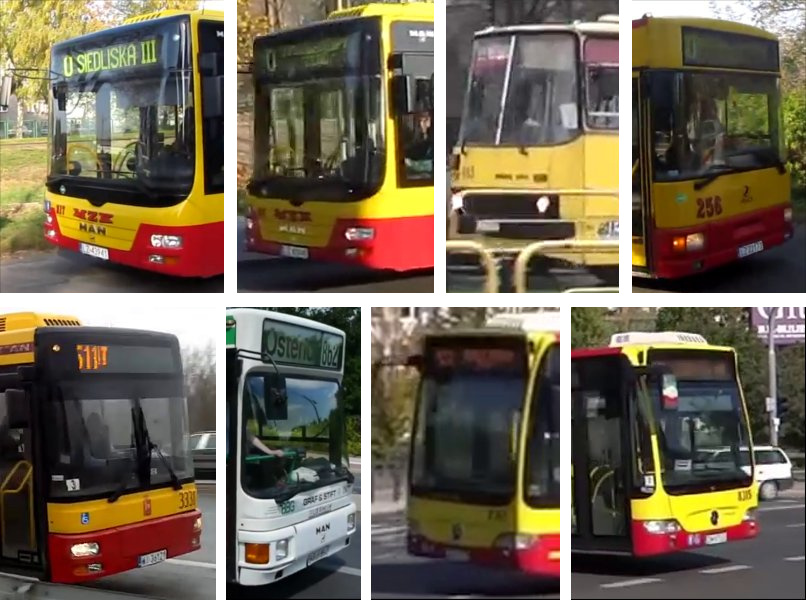
\includegraphics[width=0.8\textwidth]{img/exp_removed_distorted_fronts}
    \caption{Usunięte oznaczenia ze względu na zniekształcenia geometryczne}
    \label{fig:deformation_samples}
\end{figure}

Podsumowując, w~ramach
eksperymentów powstało 15 plików definiujących detektory, do utworzenia
których użyto zmiennych parametrów. W~pierwszej iteracji zmianie podlegały
wartości:

\begin{itemize}
\item featureType - HAAR(default), LBP, HOG,
\item minHitRate - minimalna procentowa wartość pozytywnych wykryć (domyślnie 0.995),
\item maxFalseAlarmRate - maksymalna procentowa wartość błędów (domyślnie 0.5),
\item numNeg - liczba obrazów tła do wykorzystania.
\end{itemize}

Dodatkowo powstały dwa detektory LBP osobno dla frontów typu solaris i~dla
całości zbioru (5690 wystąpień). 

W~tabeli \ref{tab:it1detectorlist} przedstawiono użyte wartości
wymienionych parametrów dla wszystkich 15 detektorów.

\begin{table}[!h]
    \centering
    \begin{tabular}{r|c|c|c|c|c|c|l}
Lp.       & Typ cech & minHitRate & maxFAR & numNeg & numPos & \%ok & błędy\\
          \hline
01        & haar     & 0.995      & 0.5       & 1000 & 2000 & 28\% &  994 \\
02        & hog      & 0.995      & 0.5       & 1000 & 2000 & 19\% &  773 \\
03        & lbp      & 0.995      & 0.5       & 1000 & 2000 & 25\% &  1738 \\
04        & lbp      & 0.995      & 0.5       & 1000 & 943  & 17\% &  143 \\
05        & lbp      & 0.995      & 0.5       & 1000 & 5960 & 91\% &  48028 \\
06        & lbp      & 0.996      & 0.5       & 1000 & 5960 & 93\% &  67711 \\
07        & lbp      & 0.997      & 0.5       & 1000 & 5960 & 93\% &  79566 \\
08        & lbp      & 0.998      & 0.5       & 1000 & 5960 & 94\% &  104771 \\
09        & lbp      & 0.999      & 0.5       & 1000 & 5960 & 95\% &  116456 \\
10        & lbp      & 0.999      & 0.4       & 1000 & 5960 & 94\% &  41187 \\
11        & lbp      & 0.999      & 0.3       & 1000 & 5960 & 90\% &  11148 \\
12        & lbp      & 0.999      & 0.2       & 1000 & 5960 & 80\% &  1694 \\
13        & lbp      & 0.999      & 0.1       & 1000 & 5960 & 71\% &  298 \\
14        & lbp      & 0.999      & 0.5       & 2000 & 5960 & 92\% &  21358 \\
15        & lbp      & 0.999      & 0.5       & 4000 & 5960 & 85\% &  2922 \\
    \end{tabular}                                                            
    \caption{Skuteczność detektorów wyszkolonych 
        dla różnych wartości parametrów narzędzia traincascade
        (pozycja 04 została wyszkolona dla frontów typu solaris)
    }
    \label{tab:it1detectorlist}
\end{table}

Pierwsze trzy pliki utworzone były na ograniczonym podzbiorze danych, gdyż
nie wszystkie próbki były wtedy opisane.

Procedura porównywania skuteczności operowała na zbiorze obrazów
reprezentujących wystąpienia frontów autobusów solaris połączonym
z~ogólnym zbiorem. Poprawne
wykrycie liczone było wtedy gdy współrzędne prostokątów wykrytego
i~oznaczonego znajdowały się w~odległości nie większej niż 25\% odpowiadającego
wymiaru prostokąta oznaczonego: dla odciętych i~rzędnych odpowiednio szerokość
i~wysokość prostokąta. Do zliczania błędnych wykryć wykorzystano ten sam zbiór.
Ze względu na ograniczenie czasowe zrezygnowano z~wykorzystania zbioru
obrazów tła. Wyniki zaprezentowano w~tabeli \ref{tab:it1detectorlist} oraz
na wykresie \ref{fig:it1detectorlist}.

\begin{figure}
\begin{center}
\begin{tikzpicture}
\begin{groupplot}[group style={group size=1 by 2},
height=5cm,width=0.8\textwidth,
legend style={at={(0.03,0.93)},anchor=north west}]
\nextgroupplot
\addplot [only marks, color=blue] table {data/15_detectors_comparison_positive_percentage.dat};

\addlegendentry{Skutecznosc}

\nextgroupplot
\addplot [only marks, color=red] table {data/15_detectors_comparison_negative_count.dat};
\addlegendentry{Bledne trafienia}
\end{groupplot}
\end{tikzpicture}
\end{center}
\caption{Zależność skuteczność i~błędnych trafień dla poszczególnych detektorów}
\label{fig:it1detectorlist}
\end{figure}

Jak widać wyniki w~większości przypadków oscylowały w~granicach 90\%.
W~odróżnieniu od poprzednich testów, te wykonane były na klatkach obrazu
w~oryginalnej rozdzielczości (wysokość 720p). 
Kolejnym krokiem było znalezienie
optymalnego czynnika skalującego. Innymi słowy jak bardzo można zmniejszyć
obraz wejściowy aby utrzymać wyniki na zadowalającym poziomie
(lub jak okazało się po przeprowadzeniu pierwszych eksperymentów,
poprawić skuteczność w~porównaniu do skuteczności detektora uruchomionego
dla obrazu w~rozmiarze oryginalnym).

\subsubsection{Skalowanie obrazu wejściowego - podsumowanie}

W~celu zmniejszenia złożoności obliczeniowej przeprowadzone zostały
testy przy przeskalowanych klatkach wejściowych. W~tym przypadku
eksperymentowano już na urządzeniu i~większość testów wykonywana była
manualnie. Metodą prób i~błędów wyznaczono parametry dla których
osiągnięto optymalne wyniki. Ostatecznie w~wersji deweloperskiej 
programu wykorzystano następujące parametry:

\begin{itemize}
    \item każdą wejściową klatkę przeskalowywano do 140 pikseli wysokości
        z~zachowaniem proporcji,
    \item minimalne wymiary szukanego obiektu to 60x60 pikseli,
    \item maksymalne 120x120 - gdy osoba stojąca na przystanku jest tuż
        przy autobusie następuje duże zniekształcenia geometryczne
        frontu. Czworokąt okalający wyznaczający front jest nieco
        przesunięty i~metoda wykrywania numeru w~lewym górnym rogu jest
        wtedy nieskuteczna.
\end{itemize}

Krok pierwszy kaskady - zawężenie poszukiwań numeru do obszaru frontu
(tymczasowo lewego-górnego fragmentu frontu) - był na tyle skuteczny,
że dalsze usprawnienia tego elementu nie były wymagane. Zasadnym było
natomiast przygotowanie zestawu testowego i~automatyczne 
przetestowanie skuteczności rozwiązania co uczynione 
zostało w~ramach drugiej iteracji.

W~procesie półautomatycznego uczenia i~oznaczania
próbek
zaobserwowano jeden szczególny trend, który faworyzował pewne
szczególne cechy frontów z~wyświetlaczem. Podczas ostatniego przebiegu
(do 5000 pozytywnych oznaczeń) zaobserwowano, że detektor
chętnie identyfikuje fronty z~diodowym wyświetlaczem zajmującym 
całą górną część frontu. Przy tak dużej liczbie oznaczeń
cechą szczególną okazał się właśnie ów wyświetlacz. Cecha ta była
na tyle istotna, że oznaczane były również fragmenty boków autobusów
z~wyświetlaczem bocznym, czy fragmenty frontów, na których wyświetlacz
nie zajmował całej długości górnej krawędzi - rysunek
\ref{fig:frontdetectormorph}.

\begin{figure}[!h]
    \centering
    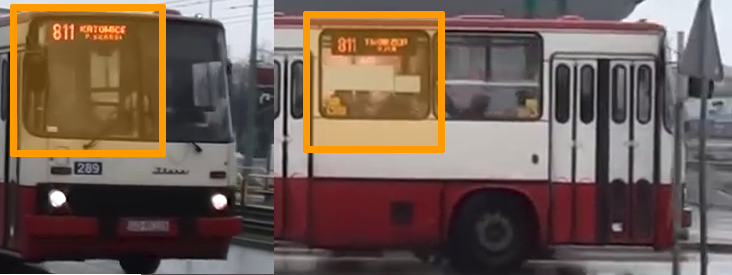
\includegraphics[width=0.95\textwidth]{img/exp_front_detector_curiosity}
    \caption{Tendencja do oznaczania fragmentów z~dużą ilością
    małych elementów w górnej części}
    \label{fig:frontdetectormorph}
\end{figure}

Możliwym rozwinięciem popełnionej implementacji jest więc przeszkolenie
detektora frontowego tak aby wykrywał również tablice boczne. Minusem
tego rozwiązania jest fakt, że z~lokalizowaniem autobusów z~tablicami
drukowanymi detektor radzi sobie znacznie gorzej. Co za tym idzie
zostały one wykluczone z~dalszych rozważań. Aby skutecznie wykrywać
fronty autobusów typu Ikarus lub starych Jelczy niezbędny byłby 
dodatkowy dedykowany detektor i~prawdopodobnie dedykowane wersje
pozostałych elementów.

\subsection{Detektor numerów}

Kaskadowy detektor wykrywający numer w~lewym górnym rogu wykrytego
frontu był jednym z~ostatnich zaimplementowanych elementów. Do wyszkolenia
detektora użyto 450 oznaczonych wystąpień numerów (jedno, dwu
i~trzycyfrowych) oraz 800 instancji tła. Ze względu na problemy podczas
szkolenia detektora dla większej liczby pozytywnych i~negatywnych 
instancji zaprzestano zwiększania ich ilości. Problem polegał na
zawieszeniu się procesu uczenia na jednym z~etapów i~gdy normalnie 
cała procedura liczona była w~dziesiątkach minut (maksymalnie 1-2 godziny)
to dla zbyt dużej liczby - w~szczególności obrazów tła proces potrafił
utknąć na danym etap na dobę.

Element ten był najsłabiej przetestowany i~wymagał usprawnienia 
w~pierwszej kolejności. Pewnym uproszczeniem było
ograniczenie obszaru przeszukiwania do lewego górnego rogu wykrytego
frontu jak na rysunku \ref{fig:frontupperleft}.

\begin{figure}[!h]
    \centering
    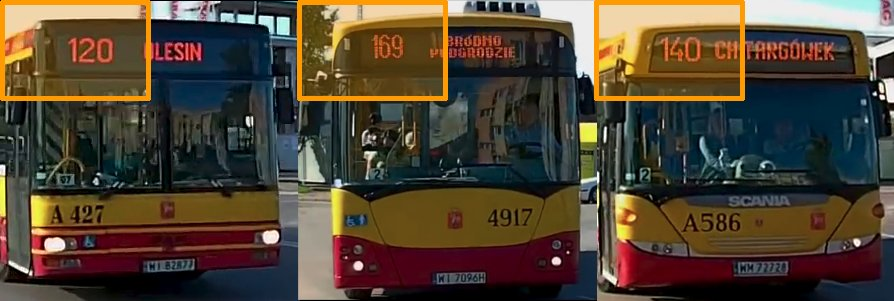
\includegraphics[width=0.95\textwidth]{img/exp_front_upper_left}
    \caption{Obszar przeszukiwany pod kątem wystąpienia numeru}
    \label{fig:frontupperleft}
\end{figure}

Możliwą alternatywą dla tego kroku była omawiana już koncepcja
oparta na detektorze MSER.

\subsection{Detektory cyfr}

W~tym podrozdziale przedstawiona została ponowna,
niespecjalnie udana próba odnalezienia optymalnych
parametrów wejściowych na proces uczenia detektora.
W~pierwszej części przedstawiono wykresy zależności pozytywnych
i~błędnych wykryć w~zależności od ilości wykorzystanych
pozytywnych próbek w~procesie uczenia. Niestety
ogromna czasochłonność przygotowywania tego typu wykresów
była główną przyczyną zaprzestania dalszych testów.
Aby przygotować pierwszą parę wykresów wyszkolono niemal 200 detektorów.
Druga para wymagała co prawda dyle samo detektorów ale większa 
liczba użytych próbek spowodowała znaczny wzrost czasu jaki był 
potrzebny do wyszkolenia poszczególnych detektorów.

\subsubsection{Cyfra 8 - szukanie optymalnych parametrów uczenia detektora}

Pierwszą cyfrą do wykrywania której szkolono detektor była cyfra 8.
Oznaczone 513 wystąpień cyfry w~scenach i~przygotowano około 2 tysiące
obrazów tła. Przy pierwszej próbie wykorzystano 100 obrazów tła, zmienną
była natomiast liczba próbek pozytywnych, która zmieniała się w~przedziale
od 10 do 200. Wyniki w~postaci ilości wykrytych poprawnie wystąpień cyfry
8, oraz błędnych wykryć przedstawiono na wykresach poniżej.

\begin{center}
\begin{tikzpicture}
\begin{groupplot}[group style={group size=1 by 2},
height=5cm,width=0.8\textwidth,
legend style={at={(0.03,0.93)},anchor=north west}]
\nextgroupplot
\addplot [only marks, color=blue] table {data/digit_8_pos_10-200_neg_100_hit_ratio.dat};

\addlegendentry{Poprawne trafienia}

\nextgroupplot
\addplot [only marks, color=red] table {data/digit_8-pos_10-200_neg_100_false_alarm_count.dat};
\addlegendentry{Bledne trafienia}
\end{groupplot}
\end{tikzpicture}
\end{center}

Pierwsze przekroczenie liczby 10 tysięcy błędnych wykryć odnotowano dla
liczby pozytywnych próbek równej 124. Pierwszym (prawdopodobnie przedwczesnym)
wnioskiem jest to, iż liczba obrazów tła powinna być
większa bądź równa liczbie próbek pozytywnych.

\begin{center}
\begin{tikzpicture}
\begin{groupplot}[group style={group size=1 by 2},
height=5cm,width=0.8\textwidth,
legend style={at={(0.03,0.93)},anchor=north west}]
\nextgroupplot
\addplot [only marks, color=blue] table {data/digit_8_pos_100-300_neg_200_hit_ratio.dat};

\addlegendentry{Poprawne trafienia}

\nextgroupplot
\addplot [only marks, color=red] table {data/digit_8-pos_100-300_neg_200_false_alarm_count.dat};
\addlegendentry{Bledne trafienia}
\end{groupplot}
\end{tikzpicture}
\end{center}

Do wykonania drugiej serii testowej wykorzystano detektory
wyszkolone przy użyciu 200 obrazów tła oraz liczby pozytywnych 
próbek w~ilości od 100 do 300 obrazów. Co łatwo zauważyć liczba 
błędnych trafień zmalała niemal o~rząd wielkości. Granica 10 tysięcy
nie została przekroczona. Dla zbioru oznaczonych 500 wystąpień cyfry 
8~najlepsze detektory nie przekroczyły liczby 400 pozytywnych trafień
więc poziom skuteczności jest nieco poniżej 80\%. Jak wiadomo
do wyszkolenia końcowej wersji detektora użyto 450 pozytywnych próbek
i~800 instancji tła.

\subsubsection{Pozostałe cyfry - podsumowanie}

Podczas przygotowywania zbiorów dla pozostałych cyfr użyto 
opisanej wcześniej metody półautomatycznego wybierania próbek pozytywnych
i~negatywnych, oraz przyrostowego uczenia detektorów z~jednoczesną
weryfikacją i~korekcją rozwiązań pośrednich. Podczas całego
procesu zaobserwowano tendencje do błędnego identyfikowania cyfr pewnej
klasy przez uczone detektory i~tak:

\begin{itemize}
    \item detektor cyfry 0 miał tendencje do wykrywania instancji cyfr
        8, 6 oraz 9,
    \item detektor cyfry 5 wykrywał również cyfry 6 oraz dużo rzadziej
        cyfry 9,
    \item detektor cyfry 2 wykrywał cyfry 4 oraz 7 itd.
\end{itemize}

Największym problemem był detektor cyfry 0, który najchętniej
wykrywał inne owalne cyfry. Najpewniejszy natomiast okazał się
detektor cyfry 1. Tym nie mniej niezbędne było wprowadzenie
mechanizmu weryfikacji potencjalnie wykrytej cyfry. Stąd 
pomysł na zastosowanie dla wykrytego fragmentu obrazu metody
Template Matching.

\subsection{Template Matching}

Przeprowadzone doświadczenie miało na celu weryfikację czy
proponowana metoda sprawdzi się w~rozwiązaniu docelowym. Dla
kilku wykrytych fragmentów wywołano funkcję pakietu OpenCV 
- \verb|matchTemplate| - i~dla zwróconych obrazów wyłuskano
minimalne i~maksymalne wartości liczbowe reprezentujące trafność
dopasowania wzorca. Okazało się, że po przeskalowaniu wykrytego
fragmentu zawierającego cyfrę do określonej wysokości, zbędne
było dopasowywanie wzorca w~różnych rozmiarach gdyż szukane cyfry
były zbliżonej wielkości. 

\begin{figure}[h!]
    \centering
    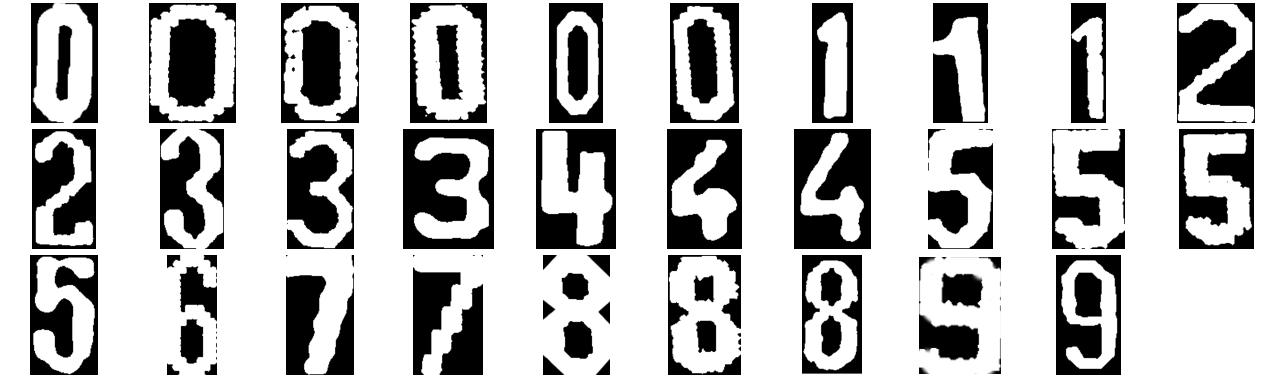
\includegraphics[width=0.95\textwidth]{img/exp_templates_used}
    \caption{Wykorzystane wzorce}
    \label{fig:used_templates}
\end{figure}

Ostatecznie w~rozwiązaniu końcowym wykorzystano wzorce zaprezentowane
na rysunku \ref{fig:used_templates}.
Przedstawione wzorce dopasowywane były bez uprzednich modyfikacji,
czego skutkiem była możliwość weryfikacji tylko jasnych cyfr
na ciemnym tle. Widać też, że niektóre cyfry były reprezentowane
przez niewiele instancji. Było to spowodowane pierwszymi testami,
a~konkretnie liniami autobusowymi jakie posłużyły w~celu
przeprowadzenia eksperymentów. Były to linie 188 oraz 523 (przystanek
Metro Politechnika 01). 

Ostatecznie niewielkim nakładem pracy można usprawnić ten etap
algorytmu poprzez dodawanie plików z~wzorcami. Przy uwzględnieniu 
konwencji nazewniczej program bez modyfikacji automatycznie
pobierał dodane pliki.

\section{Próby pierwszej wersji algorytmu - podsumowanie pierwszej iteracji}

Po przeprowadzeniu procedury szkolącej dla czterech detektorów
zaprojektowany został prosty algorytm wykrywania i~odczytywania numerów.
Algorytm składał się z~trzech etapów:

\begin{enumerate}
    \item Odszukanie frontu autobusu - wstępna segmentacja.
    \item Przyjmując założenie, że nadjeżdżający autobus jest autobusem
        nowego typu (z~wyświetlaczem diodowym), a~numer reprezentujący
        linię znajduje się w~lewym górnym rogu oznaczonego frontu,
        obszar poszukiwania numeru ograniczono do fragmentu lewej połowy
        frontu oraz pierwszej z~trzech części horyzontalnych. Na tym 
        fragmencie wyszukany został obszar reprezentujący numer -
        detektor kaskadowy podczas uczenia jako pozytywne próbki
        otrzymywał obrazy przedstawiające numery autobusów składające
        się od jednej do trzech cyfr.
    \item Na tak oznaczonym fragmencie uruchomiono dwa detektory
        dla których próbkami pozytywnymi były obrazy reprezentujące
        cyfry 1 oraz 8.
\end{enumerate}

Produktem ubocznym opisanego doświadczenia był rysunek
przedstawiający rozdzielczość wykrytego numeru w~zależności
od odległości filmowanego autobusu - rysunek \ref{fig:dist2res}.

\begin{figure}[!h]
    \centering
    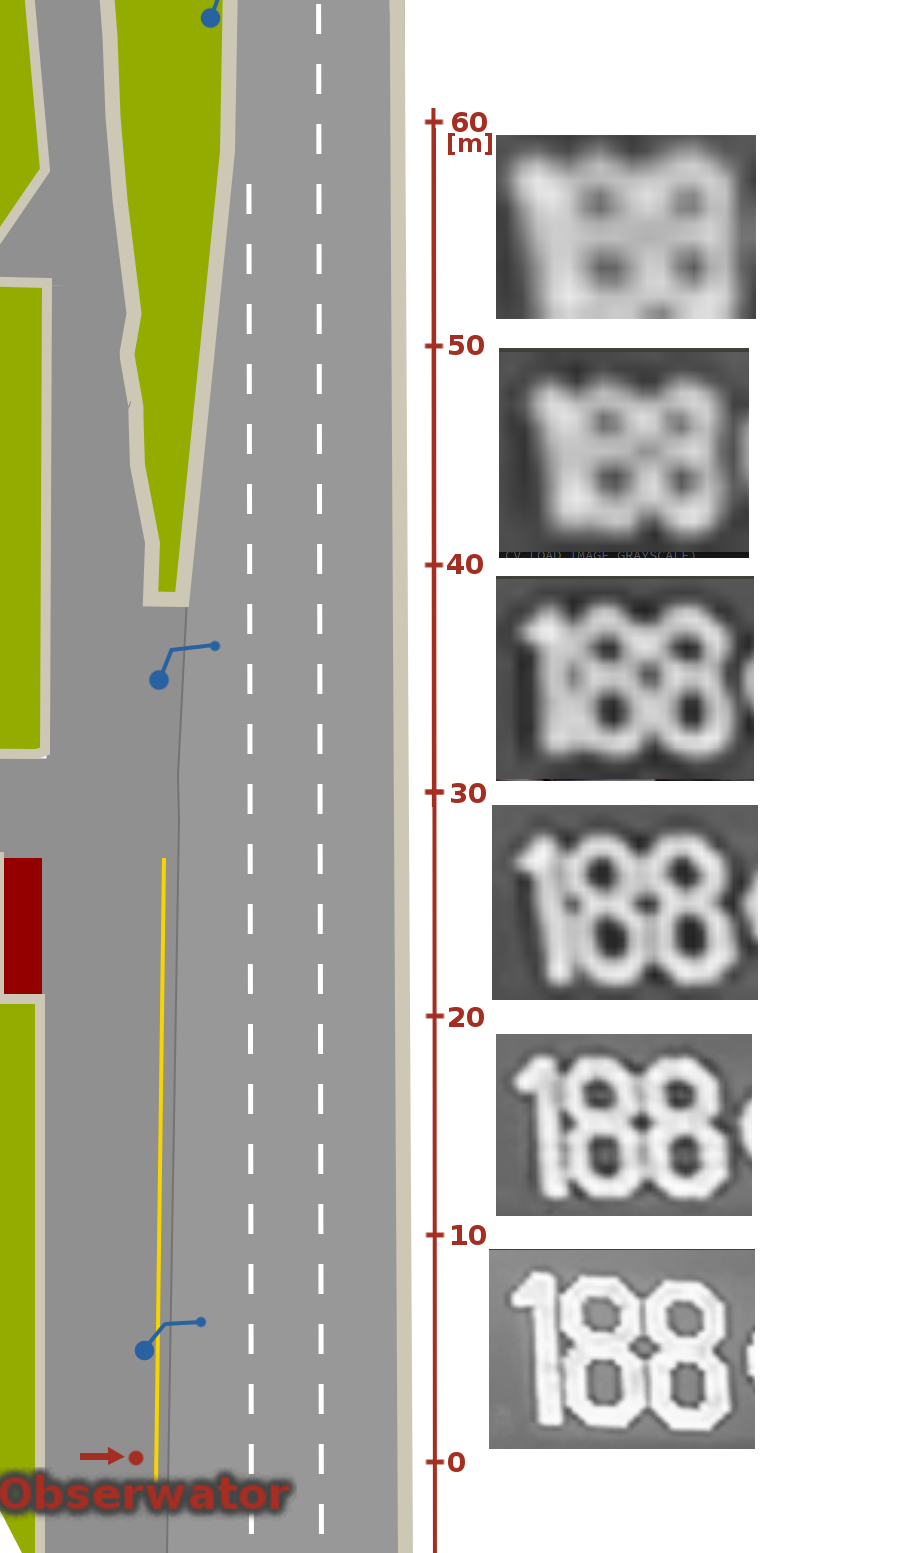
\includegraphics[height=0.9\textwidth]{img/exp_numer_od_odleglosci}
    \caption{Rozdzielczość wykrytego numeru w zależności od odległości}
    \label{fig:dist2res}
\end{figure}

Pierwszej próby dokonano dla autobusu Solaris linii 188. Odbyła się
ona na przystanku ,,Metro Politechnika 01'' w~kierunku ulicy
Marszałkowskiej.
Podczas wykonanej próby wykrycie dla detektora
odpowiedzialnego za lokalizację frontu autobusu odnotowano około dziesięć
metrów przed pierwszym zarejestrowanym wykryciem fragmentu
przedstawiającego numer linii. Niestety z tej odległości numer był
zupełnie nieczytelny. Rozdzielczość obrazu nie pozwalała na odczytanie
numeru nawet przez człowieka.
Lokalizacja fragmentu przedstawiającego numer nastąpiła gdy autobus
znajdował się w~odległości około 50m od obserwatora. Niestety
rozdzielczość na tym etapie nie pozwalała na zastosowanie jakiejkolwiek
metody segmentacji w~celu wyodrębnienia poszczególnych cyfr. Biorąc pod
uwagę dane z~rysunku \ref{fig:dist2res} segmentacja cyfr mogła by być
zastosowana dla autobusu znajdującego się w odległości mniejszej niż
30 metrów od obserwatora. 

Ostatecznie z~zarejestrowanej sekwencji wideo wyłuskano 127 obrazów
reprezentujących front autobusu. Na trzech z~nich nie zlokalizowano
numeru. 

\subsubsection{Pierwsza wersja architektury rozwiązania}

Wysokopoziomowa architektura proponowanego rozwiązania była złożona 
z~trzech etapów:
\begin{enumerate}
    \item Odnalezienie frontu autobusu - zawężenie wyszukiwania 
        do kwadratu okalającego front.
    \item Lokalizacja numeru w~obrazie reprezentującym odnaleziony
        front i~przygotowanie odseparowanego numeru jako wejścia
        do funkcji odczytującej tekst.
    \item Odczytanie numeru:
        \begin{itemize}
            \item wyszukanie potencjalnych obszarów reprezentujących
                cyfry,
            \item wyliczenie wartości reprezentującej trafność
                dopasowania cyfry w~wyznaczonym obszarze (template
                matching),
            \item wyznaczanie lokalnych maksimów oraz eliminacja 
                pozostałych teoretycznie błędnych wykryć,
            \item utworzenie ciągu znaków z~wykrytych maksimów,
                zgodnie z~kolejnością występowania w~obrazie -
                wartość odciętych lewego górnego rogu czworokąta
                okalającego.
        \end{itemize}
\end{enumerate}

\begin{figure}[!h]
    \centering
    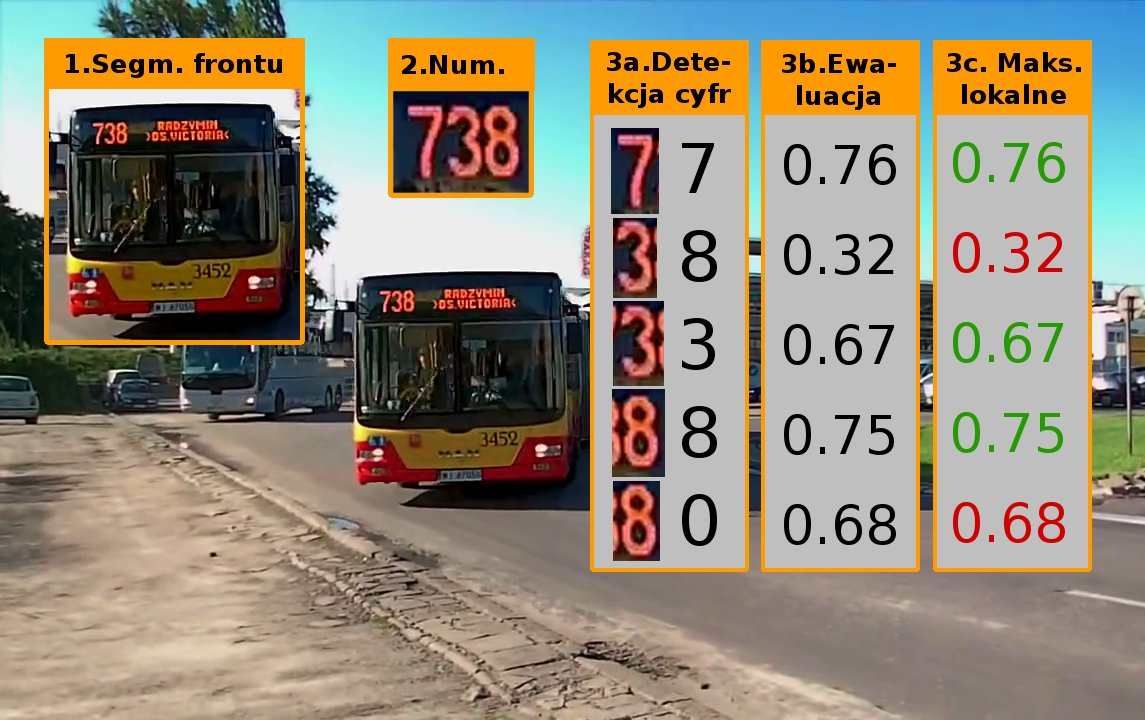
\includegraphics[width=0.9\textwidth]{img/exp_alg_explanation}
    \caption{Graficzne przedstawienie działania algorytmu na przykładzie}
    \label{fig:algexp}
\end{figure}

Rysunek \ref{fig:algexp} przedstawia przykładowy przebieg kaskady. 
Na początku wykrywany i~lokalizowany jest front autobusu.
Następnie wyłuskiwany jest fragment zawierający wyłącznie numer linii.
Ostatecznie następuje odczyt. Na zadanym fragmencie uruchamianych jest
10 detektorów dla poszczególnych cyfr. Obrazy wynikowe - potencjalnie
cyfry - przeskalowywane są do zadanej wysokości z~zachowaniem proporcji.
Dla tak przygotowanych fragmentów uruchamiana jest ewaluacja poprzez
dopasowanie wzorca lub wzorców, gdy w~zbiorze występuje kilka
reprezentacji cyfry dla różnych krojów czcionek. W~przypadku
gdy na przykład detektor trójek
wykryje ósemkę (lub na odwrót) prawdopodobnie dostanie ona niską
ocenę przy dopasowaniu tychże trójek. Ostatecznie mając
zbiór czworokątów okalających z~przypisanymi do nich wartościami
wybierane są te o~najwyższych wynikach. W~określaniu ważna jest też
odległość między cyframi. Gdyby nie wprowadzono tego kryterium
w~prezentowanym przykładzie wynik składał by się z~cyfr 7, 8 oraz 0.
Które to zero zostało wyeliminowane ze względu na zbyt bliskie położenie
względem wykrytej cyfry 8 z~wyższym wynikiem.

Aby przetestować algorytm w~praktyce
popełniono pierwsza implementację testową w~języku programowania
python z~wykorzystaniem biblioteki OpenCV w wersji 2.4.9.
Jedyny test jaki wykonano był raczej potwierdzeniem, że
rozwiązanie to może zadziałać, jednak nie wykonano testów
weryfikujących skuteczność automatu. Pierwsze rezultaty
pracy z~programem zaprezentowano na rysunku \ref{fig:finaltest}.

\begin{figure}[!h]
    \centering
    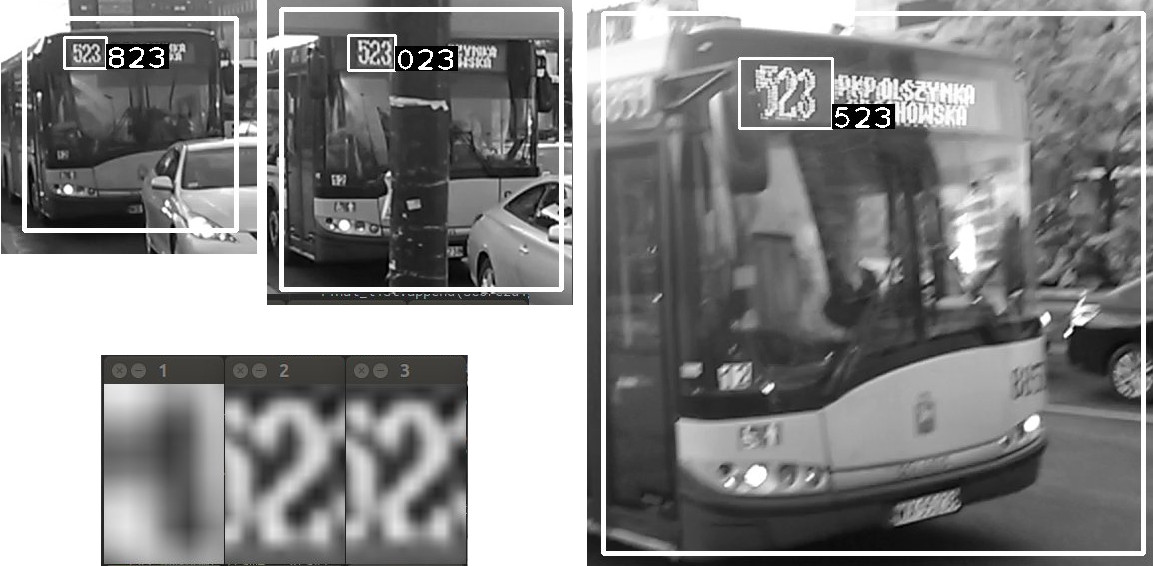
\includegraphics[width=0.9\textwidth]{img/exp_final_test}
    \caption{Ostatni test przed implementacją na telefonie}
    \label{fig:finaltest}
\end{figure}

W~lewym dolnym rogu rysunku można zaobserwować okienka prezentujące
wyniki działania detektorów do wyszukiwania cyfr. Jak nie trudno
zgadnąć były one najmniej precyzyjnym elementem całego systemu.

Jak już wspomniano był to ostatni test przed implementacją 
docelową. Jedyną zmierzoną wartością był czas potrzebny na wykrycie
frontu oraz odczytanie numeru. Na komputerze stacjonarnym z~procesorem
Intel i5 wynosił on około 100 ms na wyszukanie frontu oraz 150 ms na
odczytanie numeru. 


\section{Druga wersja algorytmu - wyniki testów porównawczych}

Po wykonaniu pierwszej implementacji programu oraz 
uruchomieniu go na urządzeniu podjęto decyzję o~ponownym 
wyszkoleniu i~przetestowaniu poszczególnych elementów systemu.
Ze względu na brak narzędzi testowych jedyne co wiadomo 
na temat pierwszej wersji to czas jaki jest potrzebny
na wykrycie i~odczytanie numeru.
Nie została ustalona skuteczność poszczególnych
elementów oraz całego systemu.

W~tym podrozdziale opisane zostały użyte parametry oraz proces
jaki został wykonany do ich ustalenia. Do uczenia detektorów
i~ich testowania wykorzystano zdjęcia pobrane z~serwisu:
\verb|www.phototrans.eu|.


\subsection{Detektor numeru}

Wykonano szereg przebiegów testowych dla zmiennych parametrów zarówno
podczas uczenia jak i~testowania. Wszystkie detektory uczone były
z~wykorzystaniem cech LBP. Pierwszym zestawem zmiennych parametrów
była ilość pozytywnych i~negatywnych próbek wykorzystanych w procesie
uczenia. Wyniki zaprezentowano w~tabeli 
\ref{tab:final_number_detector_numposneg}.

\begin{table}[!h]
    \centering
    \begin{tabular}{c|c|c|c}
        Próbki pozytywne & Obrazy tła & Skuteczność & Błędne trafienia
        \\ \hline
        1000 & 1000 & 88\% & 3860 \\
        1500 & 1500 & 90\% & 5003 \\
        2000 & 2000 & 86\% & 1034 \\
        2500 & 2500 & 86\% & 1149 \\
        2800 & 2800 & 89\% & 1186 \\
    \end{tabular}
    \caption{Skuteczność detektora oraz liczba błędnych trafień
    w~zależności od liczby próbek pozytywnych i~obrazów tła
wykorzystanych w~procesie uczenia}
    \label{tab:final_number_detector_numposneg}
\end{table}

Dalej posługiwano się detektorem wyszkolonym dla 2800 próbek pozytywnych
oraz takiej samej ilości obrazów tła. Kolejne testy ze~zmiennymi
parametrami
wykonywane były podczas procesu testowania detektorów. 
Przestrzeń poszukiwań, czyli czworokąt foremny reprezentujący
front autobusu przeskalowywano do zadanej wysokości i~szerokości.
Wyniki tych eksperymentów zaprezentowano w~tabeli 
\ref{tab:final_number_detector_resize}.
W~dalszych próbach używano przeskalowanego frontu do wymiarów
285 na 285 pikseli. Dzięki takiemu przeskalowaniu zwiększyła
się o~dziesięć procent skuteczność detektora. Uzyskano też
mniejszą liczbę błędnych trafień (ze 1186 do 968).

\begin{table}[!h]
    \centering
    \begin{tabular}{c|c|c}
        Wysokość & Skuteczność & Błędne trafienia
        \\ \hline
        300 & 96\% & 1241 \\
        295 & 96\% & 1118 \\
        290 & 96\% & 1111 \\
        285 & 96\% & >> 968 <<\\
        280 & 96\% & 876 \\
        275 & 95\% & 821 \\
        270 & 95\% & 747 \\
        265 & 94\% & 663 \\
        260 & 94\% & 560 \\
        255 & 93\% & 504 \\
        250 & 92\% & 453 \\
    \end{tabular}
    \caption{Skuteczność detektora oraz liczba błędnych trafień
    w~zależności od wysokości obrazu wejściowego}
    \label{tab:final_number_detector_resize}
\end{table}

Kolejnym testowanym parametrem był maksymalny rozmiar okna przesuwnego.
Wprowadzenie ograniczenia pozwoliło nieznacznie zmniejszyć
liczbę błędnych trafień. Zgodnie z~tabelą
\ref{tab:final_number_detector_maxsize} ograniczono 
błędne trafienia z~968 do 945. Co dziwne, dla rosnącej 
wartości maksymalnej szerokości okna, wartość błędnych
trafień rosła ponad tą, którą osiągnięto bez żadnego
ograniczenia. W~dalszych doświadczeniach maksymalną szerokość
okna ustawiono na poziomie 60 pikseli.

\begin{table}[!h]
    \centering
    \begin{tabular}{c|c|c}
        Maksymalna szerokość & Skuteczność & Błędne trafienia
        \\ \hline
        50 & 92\% & 837 \\
        55 & 96\% & 933 \\
        60 & 96\% & >> 945 << \\
        65 & 96\% & 968 \\
        75 & 96\% & 988 \\
        80 & 96\% & 1003 \\
    \end{tabular}
    \caption{Skuteczność detektora oraz liczba błędnych trafień
    w~zależności od maksymalnej szerokości okna przesuwnego}
    \label{tab:final_number_detector_maxsize}
\end{table}

Przetestowano też minimalny rozmiar okna przesuwnego.
Zgodnie z~tabelą \ref{tab:final_number_detector_minsize} ograniczono 
minimalną szerokość okna do 45 pikseli. 
Nie zmniejszyło to ilości błędnych wykryć.
Jednak dwuprocentowy spadek skuteczności 
świadczył, że ograniczenie wpływa na poprawnie wykryte numery
na co też nie można było sobie pozwolić.
W~dalszych doświadczeniach minimalną szerokość
okna ustawiono na poziomie 45 pikseli.

\begin{table}[!h]
    \centering
    \begin{tabular}{c|c|c}
        Minimalna szerokość & Skuteczność & Błędne trafienia
        \\ \hline
        44 & 96\% & >> 945 << \\
        48 & 94\% & 551 \\
        52 & 88\% & 235 \\
    \end{tabular}
    \caption{Skuteczność detektora oraz liczba błędnych trafień
    w~zależności od minimalnej szerokości okna przesuwnego}
    \label{tab:final_number_detector_minsize}
\end{table}

Ostatecznie wprowadzając ograniczenie geometryczne:
\verb|x < 85| i \verb|y < 55| gdzie \verb|x| i \verb|y| to współrzędne
lewego górnego rogu okna przesuwnego, otrzymano detektor
o~następujących właściwościach:

\begin{itemize}
    \item skuteczność 2946/3099 (prawie 95\%),
    \item ilość błędnych oznaczeń 146.
\end{itemize}

\subsection{Detektor frontu}

Po wypracowaniu optymalnych parametrów dla detektora numeru,
taką samą procedurę wykonano ponownie w~celu określenia
optymalnych parametrów dla detektora frontów autobusów 
z~numerem prezentowanym przez wyświetlacz diodowy.


\begin{figure}[h!]
\begin{center}
\begin{tikzpicture}
\begin{axis}[
    ylabel={$Trafienia$},
    xlabel={$Wysokosc\ obrazu$},
    minor y tick num=1,
    legend style={at={(0.60,0.40)},anchor=north west},
    width=\textwidth*0.6, height=6cm
]
\addplot [only marks, color=blue] table {data/front2hitra.dat};
\addlegendentry{skuteczność}
\addplot [only marks, color=red] table {data/front2false.dat};
\addlegendentry{ilość błędów}
\end{axis}
\end{tikzpicture}
\end{center}
\caption{Skuteczność w procentach oraz liczba błędnych trafień
w~zależności od wysokości obrazu wejściowego}
\label{chart:img_height2hitratio}
\end{figure}

Wysokość obrazu ustawiono na 300 pikseli. Dla~tej wartość
detektor posiadał:
\begin{itemize}
    \item skuteczność: 96\% (1829/1903),
    \item ilość błędnych trafień: 42.
\end{itemize}

Co prawda najlepszy wynik - 98\% (1862/1903) - osiągnięto dla wysokości
równej 450 pikseli, jednak trzykrotnie większa liczba błędnych
trafień oraz półtora raza większy obraz do przeszukania
przyczyniły się do pozostania przy wysokości obrazu 
wejściowego na poziomie 300 pikseli.

Wykonując kilka kolejnych serii testowych ustalono ograniczenia
rozmiaru okna przesuwnego tak aby nie było ono mniejsze niż 50
(spadek poprawnych wykryć z 1829 do 1818, oraz negatywnych 
z 42 do 29). W~przypadku instalacji aplikacji na niektórych 
urządzeniach
ze względu na niewielką rozdzielczość wbudowanych aparatów
można tę wartość jeszcze zwiększyć (możliwe że nawet dwukrotnie,
do 1/3 wysokości obrazu wejściowego). Maksymalny rozmiar
okna ustawiono na 250 pikseli.
Nie miało to wpływu na skuteczność ani~ilość błędnych
trafień. Autobus wypełniający klatkę obrazu też nie jest 
pożądany, ze względu na wysoki poziom zniekształceń geometrycznych
uniemożliwiających odczyt, spowodowanych fizyczną bliskością
czoła autobusu od soczewki aparatu.

\begin{figure}[h!]
\begin{center}
\begin{tikzpicture}
\begin{axis}[
    ylabel={$Trafienia$},
    xlabel={$Wspolczynnik\ skalujacy$},
    minor y tick num=1,
    legend style={at={(0.65,0.95)},anchor=north west},
    width=\textwidth*0.6, height=6cm
]
\addplot [only marks, color=blue] table {data/frosca2hitra.dat};
\addlegendentry{skuteczność}
\addplot [only marks, color=red] table {data/frosca2false.dat};
\addlegendentry{ilość błędów}
\addplot [only marks, color=black] table {data/frosca2effi.dat};
\addlegendentry{czas}
\end{axis}
\end{tikzpicture}
\end{center}
\caption{Skuteczność w procentach, liczba błędnych trafień
    oraz czas wykonania w~sekundach na 1903 przeskalowanych obrazów
w~zależności od współczynnika skalującego}
\label{chart:img_scale2hitratio}
\end{figure}

Po analizie wykresu \ref{chart:img_scale2hitratio}
pozostawiono współczynnik skalujący na 
domyślnym poziomie (wartość 1.1), posiadając
jednak informację, że w~razie problemów z~mocą obliczeniową
bez większego uszczerbku na skuteczności można będzie przestawić
go na 1.2 zyskując w~ten sposób kilka milisekund
(na procesorze Intel i5 dokładnie 7 ms).

\subsection{Detektor cyfr}

Eksperymentując z~detektorem cyfr i~jego parametrami wywołania
osiągnięto zaskakujący wynik. Metodą prób i~błędów ostatecznie
ustawiono parametry zgodnie z~listą:
\begin{itemize}
    \item wysokość obrazu wejściowego (numeru): 70 pikseli,
    \item parametr skalujący: 1.36,
    \item minimalna i~maksymalna wielkość okna: bez ograniczeń,
    \item minimalna liczba sąsiadów: 1.
\end{itemize}
Dla powyższych parametrów otrzymano skuteczność na poziomie 98,76\%
lecz niezwykle dużą liczbę błędnych trafień, ponad cztery tysiące
(4036).

Niestety ze względu na niewielki rozmiar obrazu wejściowego
(70 pikseli wysokości) automatyczny pomiar skuteczności
zwracał bardzo niedokładne wyniki. W~dalszych testach
zaniechano pomiaru skuteczności detektora cyfr na rzecz testów
całego rozwiązania. W~następnym (ostatnim) podrozdziale przedstawiono
porównanie skuteczności pierwotnego rozwiązania z~pierwszej iteracji
oraz wersje z~wprowadzonymi usprawnieniami.

\subsection{Testy całego algorytmu}

Po przygotowaniu zbioru 1903 obrazów zawierających fronty autobusów
z~wyświetlaczem led przystąpiono do automatycznej weryfikacji 
skuteczności pierwotnego algorytmu zaimplementowanego na urządzeniu
w~ramach pierwszej iteracji.
Pliki z~frontami autobusów posiadały numer linii w~nawie pliki. 
Na tej podstawie automat weryfikował wynik otrzymany od narzędzia
poddawanego testom.


\begin{table}[!h]
    \centering
    \begin{tabular}{c|c|c}
        Wykryte fronty  & Wykryte numeru & Poprawne odczyty \\ \hline
        1119 & 1016 & 551
    \end{tabular}
    \caption{Ilość wykrytych frontów, numerów i ogólnych poprawnych 
    odczytów pierwszej wersji algorytmu}
    \label{tab:first_version_results}
\end{table}

Wyniki zamieszczone w~tabeli \ref{tab:first_version_results}
reprezentują ilość poprawnych odczytów na próbce testowej
liczącej 1903 fronty autobusów. Końcowa skuteczność
pierwszej wersji algorytmu jest więc na poziomie 29\%.

Wykorzystując parametry detektora frontów uzyskane w~drugiej
iteracji uzyskano znacznie lepsze wyniki zaprezentowane w~tabeli
\ref{tab:second_version_results}.

\begin{table}[!h]
    \centering
    \begin{tabular}{c|c|c}
        Wykryte fronty  & Wykryte numeru & Poprawne odczyty \\ \hline
        1820 & 1609 & 845
    \end{tabular}
    \caption{Ilość wykrytych frontów, numerów i ogólnych poprawnych 
    odczytów drugiej wersji algorytmu (detektor frontów)}
    \label{tab:second_version_results}
\end{table}

Ogólna skuteczność wzrosła do 44\%. Jest to nadal kiepski wynik.
Co jest tu jednak niezwykle ważne to to, że 
poprzez poprawę jednego elementu
poprawiono ogólną skuteczność o~15\%.

Poprzez podmianę detektora numerów, na ten wytrenowany 
podczas drugiej iteracji otrzymano rezultaty widoczne
w~tabeli \ref{tab:upset_second_version_number_detector}.

\begin{table}[!h]
    \centering
    \begin{tabular}{c|c|c}
        Wykryte fronty  & Wykryte numeru & Poprawne odczyty \\ \hline
        1820 & 1517 & 764 
    \end{tabular}
    \caption{Ilość wykrytych frontów, numerów i ogólnych poprawnych 
    odczytów drugiej wersji algorytmu (detektor frontów)}
    \label{tab:upset_second_version_number_detector}
\end{table}

Pomimo wysokiej skuteczności w~teście syntetycznym
detektor numerów z~drugiej iteracji miał gorszą skuteczność
niż pierwszy prototyp. Otrzymano też dużo gorszy wynik
ogólny, bo skuteczność całego rozwiązania spadła do
40\%.

Ostatni przykład, czyli gorszy wynik dla teoretycznie 
lepszego detektora świetnie pokazuje jak ważny jest zbiór
danych, jego jakość i~co najważniejsze liczność. 
W~celu rzetelnego przebadania skuteczności zbiór danych 
rzędu kilku tysięcy to zbyt mało. Szczególnie gdy część 
z~tych danych służyła też jako zbiór uczący.
W~przypadku tak skomplikowanych obiektów wymagane są 
dane liczone w~dziesiątkach o~ile nie setkach tysięcy.
Przykładem może być publiczny zbiór danych SVHN.

Na tym etapie wstrzymano się od dalszej optymalizacji. 
Proponowane rozwiązanie wymaga jeszcze dużo pracy nad 
doskonaleniem poszczególnych jego elementów.
Jest jednak wielce prawdopodobne, że po dopracowaniu 
wszystkich kroków skuteczność będzie więcej niż zadowalająca.
